\documentclass[10pt]{article}

% NOTE: Replace this preamble with the official AAAI-27 author kit before submission.
\usepackage[margin=0.9in]{geometry}
\usepackage{times}
\usepackage{microtype}
\usepackage{amsmath,amssymb,amsfonts}
\usepackage{booktabs}
\usepackage{graphicx}
\usepackage{subcaption}
\usepackage{multirow}
\usepackage{xcolor}
\usepackage{enumitem}
\usepackage{algorithm}
\usepackage{algpseudocode}
\usepackage[numbers,sort&compress]{natbib}
\usepackage[colorlinks=true,linkcolor=blue,citecolor=blue,urlcolor=blue]{hyperref}

\graphicspath{{figures/}}
\setlength{\textfloatsep}{8pt plus 2pt minus 2pt}
\setlength{\floatsep}{8pt plus 2pt minus 2pt}
\setlength{\intextsep}{8pt plus 2pt minus 2pt}
\setlist[itemize]{leftmargin=*,topsep=2pt,itemsep=1pt}

% Placeholder macro — fill before submission
\newcommand{\todo}[1]{\textcolor{red}{\textbf{[TODO: #1]}}}

% Paper-specific macros
\newcommand{\ours}{F-CS-WAE}
\newcommand{\simple}{CS-WAE}
\newcommand{\zc}{z_{\mathrm{c}}}
\newcommand{\zs}{z_{\mathrm{s}}}
\newcommand{\muc}{\mu_{\mathrm{c}}}
\newcommand{\mus}{\mu_{\mathrm{s}}}
\newcommand{\Sph}{\mathbb{S}}
\newcommand{\R}{\mathbb{R}}
\newcommand{\MMD}{\mathrm{MMD}}
\newcommand{\CE}{\mathrm{CE}}
\newcommand{\SCauchy}{\mathrm{SCauchy}}
\newcommand{\diag}{\mathrm{diag}}

% ============================================================
\title{\vspace{-1.0em}
F-CS-WAE: Factorized Spherical Cauchy Wasserstein Auto-Encoders\\
for Label-Guided Generative Clustering
\vspace{-0.3em}}

\author{
Anonymous Authors\\
\small Anonymous Institution\\
\small \texttt{anonymous@example.com}
}
\date{}
% ============================================================

\begin{document}
\maketitle

% ============================================================
\begin{abstract}
% ============================================================
Learning a latent representation that simultaneously supports clustering,
reconstruction, and class-conditional generation is difficult because these
objectives impose conflicting pressures on the same latent space.
We present \ours{} (Factorized Class-Structured Spherical Cauchy Wasserstein
Auto-Encoder), which resolves this tension by separating the latent code into
a hyperspherical \emph{semantic} variable $\zc\in\Sph^{d_c-1}$ and a Euclidean
\emph{style} variable $\zs\in\R^{d_s}$.
The semantic latent is aligned with class-conditional Spherical Cauchy priors
via supervised MMD; the style latent is regularized toward $\mathcal{N}(0,I)$
to carry residual intra-class variation.
A four-phase training curriculum separates reconstruction learning from prior
alignment, keeping optimization stable.

On CIFAR-10, \ours{} achieves $80.87\pm0.52\%$ clustering accuracy over three seeds
with FID $83.04\pm0.86$, substantially outperforming VAE, WAE-MMD, and VaDE baselines
under the same protocol.
On MNIST, it obtains $99.15\%$ clustering accuracy and SSIM $0.983$---yet naive
class-conditional generation (sampling $\zs\sim\mathcal{N}(0,I)$ independently)
produces correct-class images only $15\%$ of the time.

We diagnose the root cause: global style MMD enforces $q(\zs)\approx\mathcal{N}(0,I)$
in aggregate but does \emph{not} prevent $q(\zs\mid y{=}k)$ from being class-specific.
Class-conditional style means in the MNIST checkpoint are separated by average
pairwise distance ${\approx}6.25$, revealing that $\zs$ carries class information
the decoder learned to exploit.
We address this with two contributions: (i)~\emph{per-class style MMD}, a
training-time regularizer that aligns each conditional style distribution to
$\mathcal{N}(0,I)$ independently, and (ii)~a \emph{class-conditional diagonal style prior}
that restores generation self-accuracy from $15\%$ to $100\%$ on the existing
checkpoint without retraining.
Our central finding is that architectural factorization does not imply statistical
independence---the sampling distribution must match the conditional structure the
representation actually learned.
\end{abstract}

% ============================================================
\section{Introduction}
% ============================================================

Auto-encoding generative models serve three masters simultaneously.
\emph{Reconstruction} rewards retaining all information needed to reproduce an input.
\emph{Clustering} rewards removing nuisance variation so that examples from the same
class form compact, well-separated groups.
\emph{Prior sampling} rewards aligning the encoded representation to a distribution
from which new codes can be drawn and decoded into realistic images.
Optimizing one objective can silently damage the others: a representation can form
clean clusters while generating poor prior samples, or reconstruct inputs accurately
while providing no class structure.

This tension is apparent in standard models.
Variational auto-encoders (VAEs)~\citep{kingma2013autoencoding} provide probabilistic
priors but their Euclidean Gaussian posteriors do not organize class structure.
Wasserstein auto-encoders (WAEs)~\citep{tolstikhin2017wasserstein} match the
aggregated posterior to a prior using MMD or adversarial objectives, but global
aggregate matching says nothing about per-class structure.
VaDE~\citep{jiang2016variational} introduces a Gaussian mixture prior for clustering
but remains Euclidean and does not separate class semantics from within-class style.

\paragraph{Factorized latent space.}
We propose \ours, which addresses the three-way tension by assigning distinct roles
to two separate latent variables.
The \emph{semantic latent} $\zc\in\Sph^{d_c-1}$ lives on a hypersphere and is
aligned with class-conditional Spherical Cauchy priors via a supervised MMD term:
examples from class $k$ are pushed toward $p(\zc\mid y{=}k)=\SCauchy(m_k,\rho_p)$.
The \emph{style latent} $\zs\in\R^{d_s}$ lives in Euclidean space and is regularized
toward $\mathcal{N}(0,I)$ to carry residual appearance variation.
Both variables are concatenated as decoder input, so the decoder can use color,
texture, and pose from $\zs$ without polluting the semantic direction $\zc$.
Clustering is performed exclusively on $\muc$, the deterministic semantic direction.

On CIFAR-10 this separation produces stable, strong clustering ($80.87\pm0.52\%$
ACC over three seeds) while maintaining favorable FID relative to all available
baselines.

\paragraph{The generation failure on MNIST.}
A natural expectation is that the factorized model would perform even better on
MNIST, where classes are visually simpler and more distinct.
It does achieve $99.15\%$ clustering accuracy and SSIM $0.983$.
But class-conditional prior samples---generated by sampling $\zc$ from the class
Spherical Cauchy prior and $\zs$ independently from $\mathcal{N}(0,I)$---decode
as the correct class only $15\%$ of the time.
The single-latent \simple{} baseline, which has weaker clustering ($87.35\%$ ACC),
produces clearly recognizable digits with FID $26.95$.

\paragraph{Diagnosis: marginal matching $\neq$ conditional independence.}
We show that the failure is structural, not incidental.
Encoding 2{,}048 MNIST test images with the trained checkpoint reveals that the
global style distribution is well-matched to $\mathcal{N}(0,I)$
(multi-scale MMD $\approx 0.0017$), yet class-conditional style means are separated
by average pairwise distance $\approx 6.25$.
The global style MMD enforces $q(\zs)\approx\mathcal{N}(0,I)$ in aggregate but
says nothing about the conditional distributions $q(\zs\mid y{=}k)$.
The decoder learns to exploit the fact that encoded $(\zc,\zs)$ pairs always come
from the same image and therefore share class information.
At generation time, independently sampled $\zc$ and $\zs$ may encode different classes,
producing combinations the decoder has never seen.

This failure is not specific to \ours: it applies to any factorized WAE whose style
regularizer operates only on the marginal distribution.

\paragraph{Proposed fixes.}
We introduce two complementary corrections.
First, \emph{per-class style MMD} ($\mathcal{L}_{\mathrm{style\text{-}cls}}$) is a
training-time regularizer that aligns each conditional style distribution
$q(\zs\mid y{=}k)$ to $\mathcal{N}(0,I)$ independently, directly preventing the
class-dependent style structure that causes generation failure.
Second, for the existing checkpoint, we show that a
\emph{class-conditional diagonal style prior}---sampling
$\zs\sim\mathcal{N}(\bar\mu_{s,k},\tau^2\,\diag(\bar\sigma_{s,k}^2))$ rather than
$\mathcal{N}(0,I)$---raises generation self-accuracy from $15\%$ to $100\%$
without any retraining.

\paragraph{Contributions.}
\begin{itemize}
  \item We propose \ours{}, a factorized label-guided WAE with a hyperspherical
        Spherical Cauchy semantic latent and a Euclidean Gaussian style latent,
        trained with a four-phase curriculum and EMA class center updates
        (Section~\ref{sec:method}).
  \item We demonstrate strong and stable clustering on CIFAR-10
        ($80.87\pm0.52\%$ ACC, three seeds) with large margins over
        VAE, WAE-MMD, and VaDE (Section~\ref{sec:cifar10}).
  \item We identify \emph{conditional style mismatch} as a failure mode for
        factorized WAEs: global style MMD does not imply class-conditional style
        independence, and this causes naive prior sampling to fail
        (Section~\ref{sec:diagnosis}).
  \item We propose \emph{per-class style MMD}, a supervised training-time
        regularizer that directly enforces conditional style independence
        (Section~\ref{sec:method}).
  \item We show that a class-conditional diagonal style prior repairs generation
        post-hoc, raising MNIST self-accuracy from $15\%$ to $100\%$, and we
        evaluate a spectrum of representation-aware sampling strategies
        (Section~\ref{sec:sampling}).
\end{itemize}

% ============================================================
\section{Related Work}
% ============================================================

\paragraph{Variational and Wasserstein auto-encoders.}
VAEs~\citep{kingma2013autoencoding} maximize an evidence lower bound that includes a
KL penalty toward a Gaussian prior.
WAEs~\citep{tolstikhin2017wasserstein} relax per-example KL to a global discrepancy
between the aggregated posterior and the prior, enabling deterministic encoders.
MMD-based WAEs use kernel two-sample tests~\citep{gretton2012kernel} as the
discrepancy; sliced-Wasserstein AEs~\citep{kolouri2018sliced} use projected
one-dimensional distances.
All match the \emph{marginal} style distribution; our per-class style MMD
additionally matches the \emph{conditional} distributions, which is necessary for
class-conditional generation.

\paragraph{Deep generative clustering.}
DEC~\citep{xie2015unsupervised} refines embeddings by minimizing KL divergence to
soft cluster assignments.
VaDE~\citep{jiang2016variational} introduces a Gaussian mixture latent prior that
integrates clustering into the generative model.
\ours{} differs by using labels during training (label-guided rather than fully
unsupervised) and by encoding class structure on a hypersphere rather than in a
Euclidean mixture.

\paragraph{Hyperspherical latent variables.}
S-VAE~\citep{davidson2018hyperspherical} replaces the Gaussian posterior with a
von Mises-Fisher distribution on $\Sph^{d-1}$, motivating directional latent geometry.
Spherical Cauchy VAEs~\citep{sablica2025hyperspherical} provide a heavier-tailed
spherical distribution with a Möbius-transform reparameterization that \ours{}
adopts for the semantic latent.
Spherical sliced-Wasserstein distances~\citep{bonet2022spherical} extend optimal
transport to the sphere.
\ours{} combines spherical geometry for the semantic variable with WAE-style MMD
and label-guided class priors.

\paragraph{Factorization and disentanglement.}
FactorVAE~\citep{kim2018disentangling} and $\beta$-TCVAE~\citep{chen2018isolating}
penalize total correlation to encourage statistically independent factors.
InfoGAN~\citep{chen2016infogan} uses mutual information to make latent codes
interpretable.
These approaches regularize joint distributions, but like global style MMD, they do
not explicitly target class-conditional dependence.
Our per-class style MMD is a supervised analogue: it directly penalizes the
specific dependence $\zs\not\perp y$ that causes our observed failure.

% ============================================================
\section{Method}
\label{sec:method}
% ============================================================

\subsection{Problem Setting}

Let $\mathcal{D}=\{(x_i,y_i)\}_{i=1}^{n}$ be a labeled image dataset with $K$ classes.
We seek a model satisfying three criteria simultaneously:
\begin{enumerate}[leftmargin=*]
  \item \textbf{Reconstruction.} $x\mapsto\hat{x}$ preserves visual content.
  \item \textbf{Clustering.} A simple method on semantic codes recovers class structure
        without using labels.
  \item \textbf{Class-conditional generation.} Drawing latent codes from class priors
        and decoding produces class-consistent images.
\end{enumerate}
We call this \emph{label-guided generative clustering}.
Labels structure the training objective but are not used during clustering evaluation.

\subsection{Factorized Architecture}

\paragraph{Encoder.}
A shared ResNet-18 backbone extracts features $h=f_\phi(x)$, followed by a
256-unit fully-connected layer with SiLU activation.
Two specialized heads produce the latent distribution parameters:
\begin{equation}
  E_\phi(x) = \bigl(\tilde{\muc},\;r_c,\;\mus,\;\log\sigma_s^2\bigr).
\end{equation}

The semantic direction is $\ell_2$-normalized and the concentration parameter is
bounded to $(0,1)$:
\begin{equation}
  \muc = \frac{\tilde{\muc}}{\|\tilde{\muc}\|_2},
  \qquad
  \rho_c = \sigma(r_c)(1-\varepsilon),
  \label{eq:semantic-head}
\end{equation}
where $\varepsilon=10^{-8}$ prevents $\rho_c$ from reaching its boundary.
The semantic latent is sampled by the Spherical Cauchy Möbius
reparameterization~\citep{sablica2025hyperspherical}:
\begin{equation}
  \eta_c\sim\mathrm{Unif}(\Sph^{d_c-1}),
  \qquad
  \zc = T_{\muc,\rho_c}(\eta_c).
  \label{eq:sc-reparam}
\end{equation}
The style latent uses a standard Gaussian reparameterization:
\begin{equation}
  \varepsilon_s\sim\mathcal{N}(0,I),
  \qquad
  \zs = \mus + \sigma_s \odot \varepsilon_s.
  \label{eq:style-reparam}
\end{equation}
The style log-variance head is zero-initialized ($\sigma_s\approx 1$ at start)
and logvar is clamped to $[-10, 10]$ during sampling.

\paragraph{Decoder.}
Both variables are concatenated and decoded:
\begin{equation}
  \hat{x} = D_\theta([\zc;\,\zs]).
  \label{eq:decoder}
\end{equation}
The decoder is a residual upsampling network: a linear layer reshapes $[\zc;\zs]$
to $(512,4,4)$, then three ResBlockUp stages
($512\to256\to128\to64$ channels) upsample to $32\times32$.
No skip connections are used from the encoder; the decoder depends entirely on the
latent code.

In all experiments $d_c=64$ and $d_s=128$.

\subsection{Class-Conditional Semantic Prior}

For each class $k$, \ours{} maintains $R$ center directions on the hypersphere:
\begin{equation}
  m_{k,r}\in\Sph^{d_c-1}, \quad k=1,\dots,K,\quad r=1,\dots,R.
\end{equation}
All experiments use $R=1$.
The class-conditional semantic prior is:
\begin{equation}
  p(\zc\mid y{=}k) = \SCauchy(m_k,\,\rho_p), \qquad \rho_p = 0.7.
  \label{eq:class-prior}
\end{equation}
Class center directions are updated by exponential moving average (EMA) from
batch-accumulated class-mean semantic directions, once per epoch:
\begin{equation}
  m_k \leftarrow \mathrm{normalize}\!\bigl(\tau\,m_k + (1-\tau)\,\bar\muc^{(k)}\bigr),
  \quad \tau=0.95,
  \label{eq:ema-update}
\end{equation}
where $\bar\muc^{(k)}$ is the mean $\muc$ over all examples with label $k$ in the
current epoch.
EMA updates avoid gradient competition between the decoder and the prior centers.

\subsection{Loss Terms}
\label{sec:losses}

\paragraph{Reconstruction.}
\begin{equation}
  \mathcal{L}_{\mathrm{rec}}
  = \lambda_1\|x-\hat{x}\|_1
  + \lambda_{\mathrm{LPIPS}}\,\mathrm{LPIPS}(x,\hat{x}),
  \label{eq:rec}
\end{equation}
with $\lambda_1=1.0$ and $\lambda_{\mathrm{LPIPS}}=0.1$.

\paragraph{Supervised class MMD.}
For each class $k$, let $Q_k=\{\zc^i:y_i=k\}$ be the batch of encoded semantic
samples and $P_k\sim p(\zc\mid y{=}k)$ be prior samples of equal size:
\begin{equation}
  \mathcal{L}_{\mathrm{class}}
  = \frac{1}{K}\sum_{k=1}^{K}\MMD^2(Q_k,P_k).
  \label{eq:class-mmd}
\end{equation}
The kernel is a spherical RBF $\kappa(u,v)=\exp(-\|u-v\|^2/(2\sigma^2))$
with $\sigma$ set per-batch by the median heuristic.
This term pushes class-conditional encoded distributions toward their priors.

\paragraph{Aggregated semantic MMD.}
The aggregated prior $p(\zc)=\tfrac{1}{K}\sum_k p(\zc\mid y{=}k)$ is approximated
by sampling class indices uniformly:
\begin{equation}
  \mathcal{L}_{\mathrm{agg}}
  = \MMD^2\!\Bigl(\{\zc^i\}_{i=1}^{b},\;
    \{z_{c,r_j}^p : r_j\sim\mathrm{Unif}(1,\dots,K)\}_{j=1}^{b}\Bigr).
  \label{eq:agg-mmd}
\end{equation}
This ensures global sampleability of the semantic prior.

\paragraph{Global style MMD.}
\begin{equation}
  \mathcal{L}_{\mathrm{style}}
  = \MMD_{\mathrm{RBF}}\!\Bigl(\{\zs^i\}_{i=1}^{b},\;
    \{\varepsilon_j:\varepsilon_j\sim\mathcal{N}(0,I)\}_{j=1}^{b}\Bigr).
  \label{eq:style-mmd}
\end{equation}
A multi-scale Euclidean RBF kernel with fixed bandwidths
$\{0.5, 1, 2, 5, 10, 20, 50\}$ is used to remain sensitive across a wide variance
range (median heuristic can saturate when style variance is large).

\paragraph{Per-class style MMD (proposed).}
The global term $\mathcal{L}_{\mathrm{style}}$ matches the marginal distribution
$q(\zs)$ but does not constrain the conditional distributions $q(\zs\mid y{=}k)$.
We introduce a per-class style regularizer that directly addresses this:
\begin{equation}
  \mathcal{L}_{\mathrm{style\text{-}cls}}
  = \frac{1}{K}\sum_{k=1}^{K}
    \MMD_{\mathrm{RBF}}\!\Bigl(
      \{\zs^i:y_i=k\},\;
      \{\varepsilon_j:\varepsilon_j\sim\mathcal{N}(0,I)\}_{|y_i=k|}
    \Bigr).
  \label{eq:style-cls-mmd}
\end{equation}
This term forces each class-conditional style distribution to match $\mathcal{N}(0,I)$,
preventing $\zs$ from carrying class-identifying information and making
independent style sampling reliable at generation time.

\paragraph{Auxiliary classifier.}
A linear layer $h$ on the semantic direction prevents collapse and accelerates
class organization:
\begin{equation}
  \mathcal{L}_{\mathrm{cls}} = \CE(h(\muc),\,y).
  \label{eq:cls}
\end{equation}
Used only during training; not used for clustering evaluation.

\paragraph{Total objective.}
\begin{align}
  \mathcal{L}
  &= \mathcal{L}_{\mathrm{rec}}
   + \alpha(t)\,\mathcal{L}_{\mathrm{class}}
   + \beta(t)\,\mathcal{L}_{\mathrm{agg}} \nonumber\\
  &\quad + \gamma(t)\,\mathcal{L}_{\mathrm{style}}
   + \delta(t)\,\mathcal{L}_{\mathrm{style\text{-}cls}}
   + \eta(t)\,\mathcal{L}_{\mathrm{cls}},
  \label{eq:total}
\end{align}
where the time-varying coefficients implement the training schedule below.

\subsection{Four-Phase Training Schedule}

Training proceeds in four phases to prevent early regularization from destroying
reconstruction quality:
\begin{itemize}
  \item \textbf{Phase A} (epochs 0--49):
        $\mathcal{L}_{\mathrm{rec}}$ only.
        The decoder learns a useful image manifold before any latent pressure is applied.
  \item \textbf{Phase B} (epochs 50--99):
        Add $\mathcal{L}_{\mathrm{style}}$, $\mathcal{L}_{\mathrm{style\text{-}cls}}$,
        and $\mathcal{L}_{\mathrm{cls}}$ with linear ramp-up.
        Style latents begin matching $\mathcal{N}(0,I)$ per-class; semantic codes are
        loosely anchored by the classifier.
  \item \textbf{Phase C} (epochs 100--199):
        Add $\mathcal{L}_{\mathrm{class}}$ and $\mathcal{L}_{\mathrm{agg}}$ ramping
        to half their final weight.
        Class-conditional semantic organization begins.
  \item \textbf{Phase D} (epochs 200--299):
        All terms ramp to final weight.
        The model jointly optimizes reconstruction, class-aligned semantics, and
        class-independent style.
\end{itemize}

\begin{algorithm}[t]
\caption{\ours{} training iteration}
\label{alg:fcswae}
\begin{algorithmic}[1]
\Require Batch $(x,y)$; encoder $E_\phi$; decoder $D_\theta$; classifier $h$;
         EMA centers $\{m_k\}$; phase weights $\alpha,\beta,\gamma,\delta,\eta$
\State $(\muc,\rho_c,\mus,\log\sigma_s^2)\leftarrow E_\phi(x)$
\State $\zc\leftarrow T_{\muc,\rho_c}(\eta_c)$, $\;\eta_c\sim\mathrm{Unif}(\Sph^{d_c-1})$
\State $\zs\leftarrow \mus+\sigma_s\odot\varepsilon_s$, $\;\varepsilon_s\sim\mathcal{N}(0,I)$
\State $\hat{x}\leftarrow D_\theta([\zc;\zs])$
\State Compute $\mathcal{L}$ from Eq.~\ref{eq:total}
\State Update $\phi,\theta,h$ by gradient descent on $\mathcal{L}$
\State Accumulate $(\muc,y)$ for EMA update; update $\{m_k\}$ after epoch
\end{algorithmic}
\end{algorithm}

\subsection{Inference and Generation}

\paragraph{Clustering.}
K-means is applied to the deterministic semantic directions $\muc$, followed by
Hungarian matching to compute ACC, NMI, and ARI.
Labels are not used during K-means.

\paragraph{Class-conditional generation: naive prior.}
\begin{equation}
  \zc\sim p(\zc\mid y{=}k), \quad
  \zs\sim\mathcal{N}(0,I), \quad
  \hat{x}=D_\theta([\zc;\zs]).
  \label{eq:naive-gen}
\end{equation}
This prior is reliable when per-class style MMD is used during training.

\paragraph{Class-conditional generation: conditional style prior.}
When per-class style MMD is not used (or as a post-hoc correction), estimate
class style statistics from encoded training samples:
\begin{equation}
  \bar\mus^{(k)} = \mathbb{E}[\mus\mid y{=}k],
  \quad
  \bar\sigma_s^{2(k)} = \mathrm{Var}[\mus\mid y{=}k].
  \label{eq:class-style-stats}
\end{equation}
Then sample with temperature $\tau$:
\begin{equation}
  \zs\sim\mathcal{N}\!\bigl(
    \bar\mus^{(k)},\;
    \tau^2\,\diag(\bar\sigma_s^{2(k)})
  \bigr).
  \label{eq:cond-style-prior}
\end{equation}
We find $\tau=0.25$ gives clean, class-consistent samples with controlled diversity.

% ============================================================
\section{Experiments}
% ============================================================

\subsection{Setup}

\paragraph{Datasets.}
CIFAR-10~\citep{krizhevsky2009learning} ($3\times32\times32$, $K=10$) is the primary
benchmark.
MNIST~\citep{lecun1998gradient} ($1\times32\times32$, resized, $K=10$) is used for
diagnostic analysis.
Fashion-MNIST~\citep{xiao2017fashion} will be added as the third benchmark in the
final submission.

\paragraph{Baselines.}
We compare against: ResNetAE (deterministic AE with ResNet-18 encoder), VAE,
WAE-MMD, VaDE, and the single-latent \simple{} (one Spherical Cauchy semantic
latent, no style variable, trained with the same backbone and schedule).

\paragraph{Metrics.}
\emph{Clustering:} ACC (K-means + Hungarian matching), NMI, ARI.
\emph{Reconstruction:} SSIM, PSNR, LPIPS~\citep{zhang2018unreasonable}.
\emph{Sample quality:} FID~\citep{heusel2017gans} using 10{,}000 generated and
10{,}000 real images.
\emph{Generation self-accuracy:} generated images re-encoded through the trained
auxiliary classifier; the target class is the one used to sample $\zc$.

\subsection{CIFAR-10 Main Results}
\label{sec:cifar10}

Table~\ref{tab:cifar-main} reports per-seed and aggregate CIFAR-10 results for
\ours{} over three random seeds.
Clustering is highly stable: ACC varies by only $0.52$ percentage points and FID
by less than one point, confirming that the learned semantic space is reproducible.

\begin{table}[t]
\centering
\caption{CIFAR-10 \ours{} results over three seeds.
         Higher ACC/NMI/ARI/SSIM/PSNR and lower FID/LPIPS are better.}
\label{tab:cifar-main}
\begin{tabular}{lrrrrrrr}
\toprule
Seed & ACC & NMI & ARI & SSIM & PSNR & LPIPS & FID \\
\midrule
0 & 0.8043 & 0.6426 & 0.6259 & 0.7073 & 21.88 & 0.2126 & 83.83 \\
1 & 0.8160 & 0.6607 & 0.6452 & 0.6967 & 21.67 & 0.2183 & 83.45 \\
2 & 0.8059 & 0.6455 & 0.6264 & 0.7060 & 21.76 & 0.2137 & 81.85 \\
\midrule
\textbf{Mean} & \textbf{0.8087} & \textbf{0.6496} & \textbf{0.6325}
              & 0.7034 & 21.77 & 0.2149 & \textbf{83.04} \\
Std           & 0.0052 & 0.0079 & 0.0090 & 0.0047 & 0.09 & 0.0025 & 0.86 \\
\bottomrule
\end{tabular}
\end{table}

\begin{figure}[t]
\centering
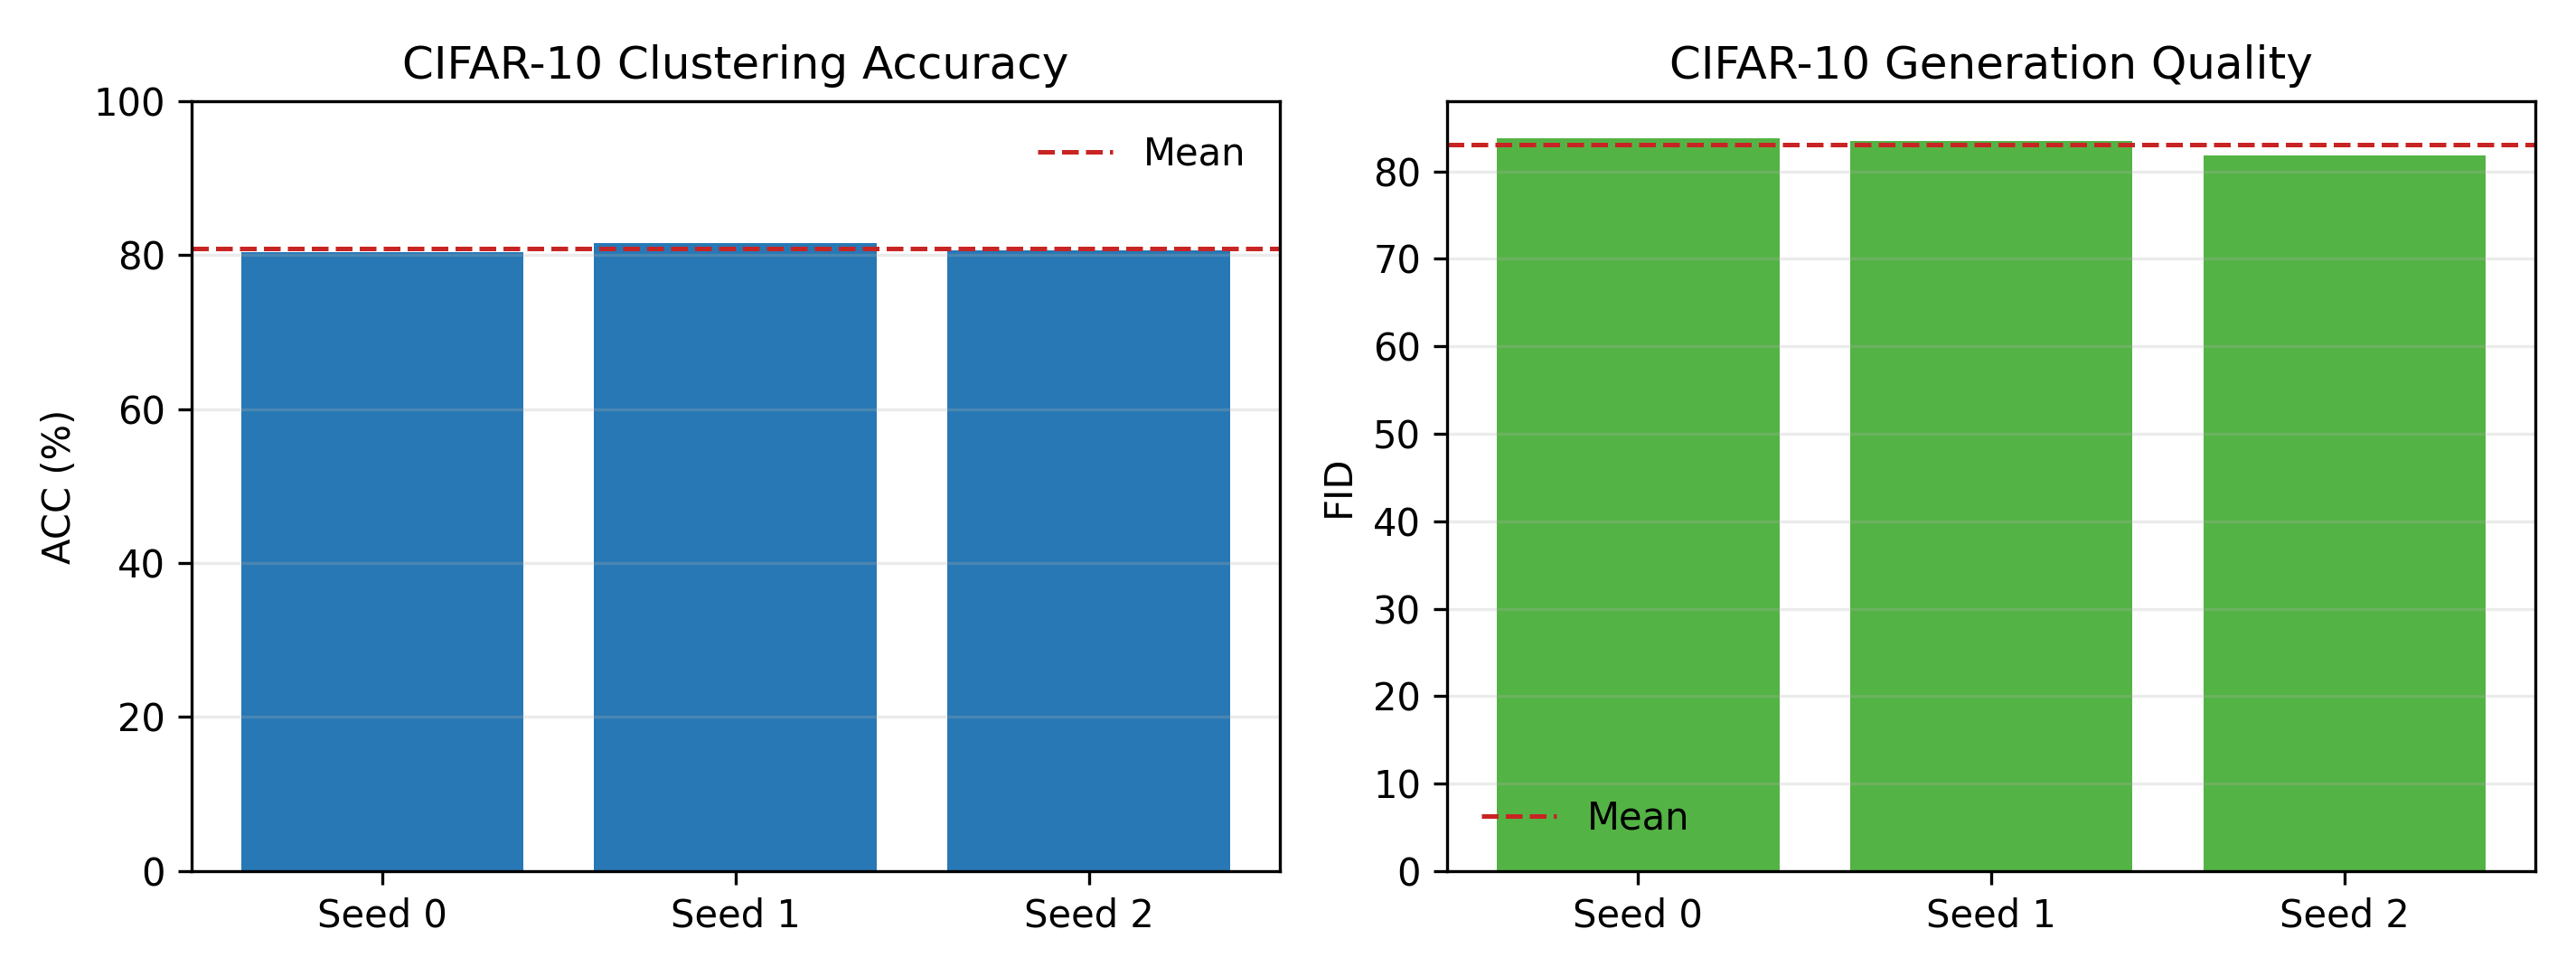
\includegraphics[width=0.95\linewidth]{cifar10_main_metrics.png}
\caption{CIFAR-10 clustering and FID across three \ours{} seeds.
         Variance is low in all metrics.}
\label{fig:cifar-main}
\end{figure}

Table~\ref{tab:cifar-baselines} compares \ours{} against available baselines on
CIFAR-10.
The ACC gap is large: ${\approx}59$ percentage points over VAE and WAE-MMD,
${\approx}66$ over VaDE.
\ours{} also achieves the best FID by a large margin.

\begin{table}[t]
\centering
\caption{CIFAR-10 comparison.
         \ours{} is a 3-seed mean; baselines are seed-0 results.
         \todo{Re-run baselines for seeds 1 and 2 and report mean$\pm$std.}}
\label{tab:cifar-baselines}
\begin{tabular}{lrrrr}
\toprule
Method & ACC $\uparrow$ & NMI $\uparrow$ & ARI $\uparrow$ & FID $\downarrow$ \\
\midrule
\textbf{\ours{} (3-seed)} & \textbf{0.8087} & \textbf{0.6496} & \textbf{0.6325} & \textbf{83.04} \\
ResNetAE & 0.2202 & 0.1017 & 0.0493 & 121.01 \\
VAE      & 0.2220 & 0.0955 & 0.0511 & 179.98 \\
WAE-MMD  & 0.2099 & 0.0979 & 0.0469 & 235.43 \\
VaDE     & 0.1475 & 0.0427 & 0.0151 & 475.87 \\
\bottomrule
\end{tabular}
\end{table}

Figure~\ref{fig:cifar-samples} shows class-conditional prior samples from the
seed-0 CIFAR-10 checkpoint.
Figure~\ref{fig:cifar-style} probes the factorization by holding $\zc$ fixed while
varying $\zs$ (columns) and holding $\zs$ fixed while varying $\zc$ (rows),
showing that both variables contribute to the decoded image in interpretable ways.

\begin{figure}[t]
\centering
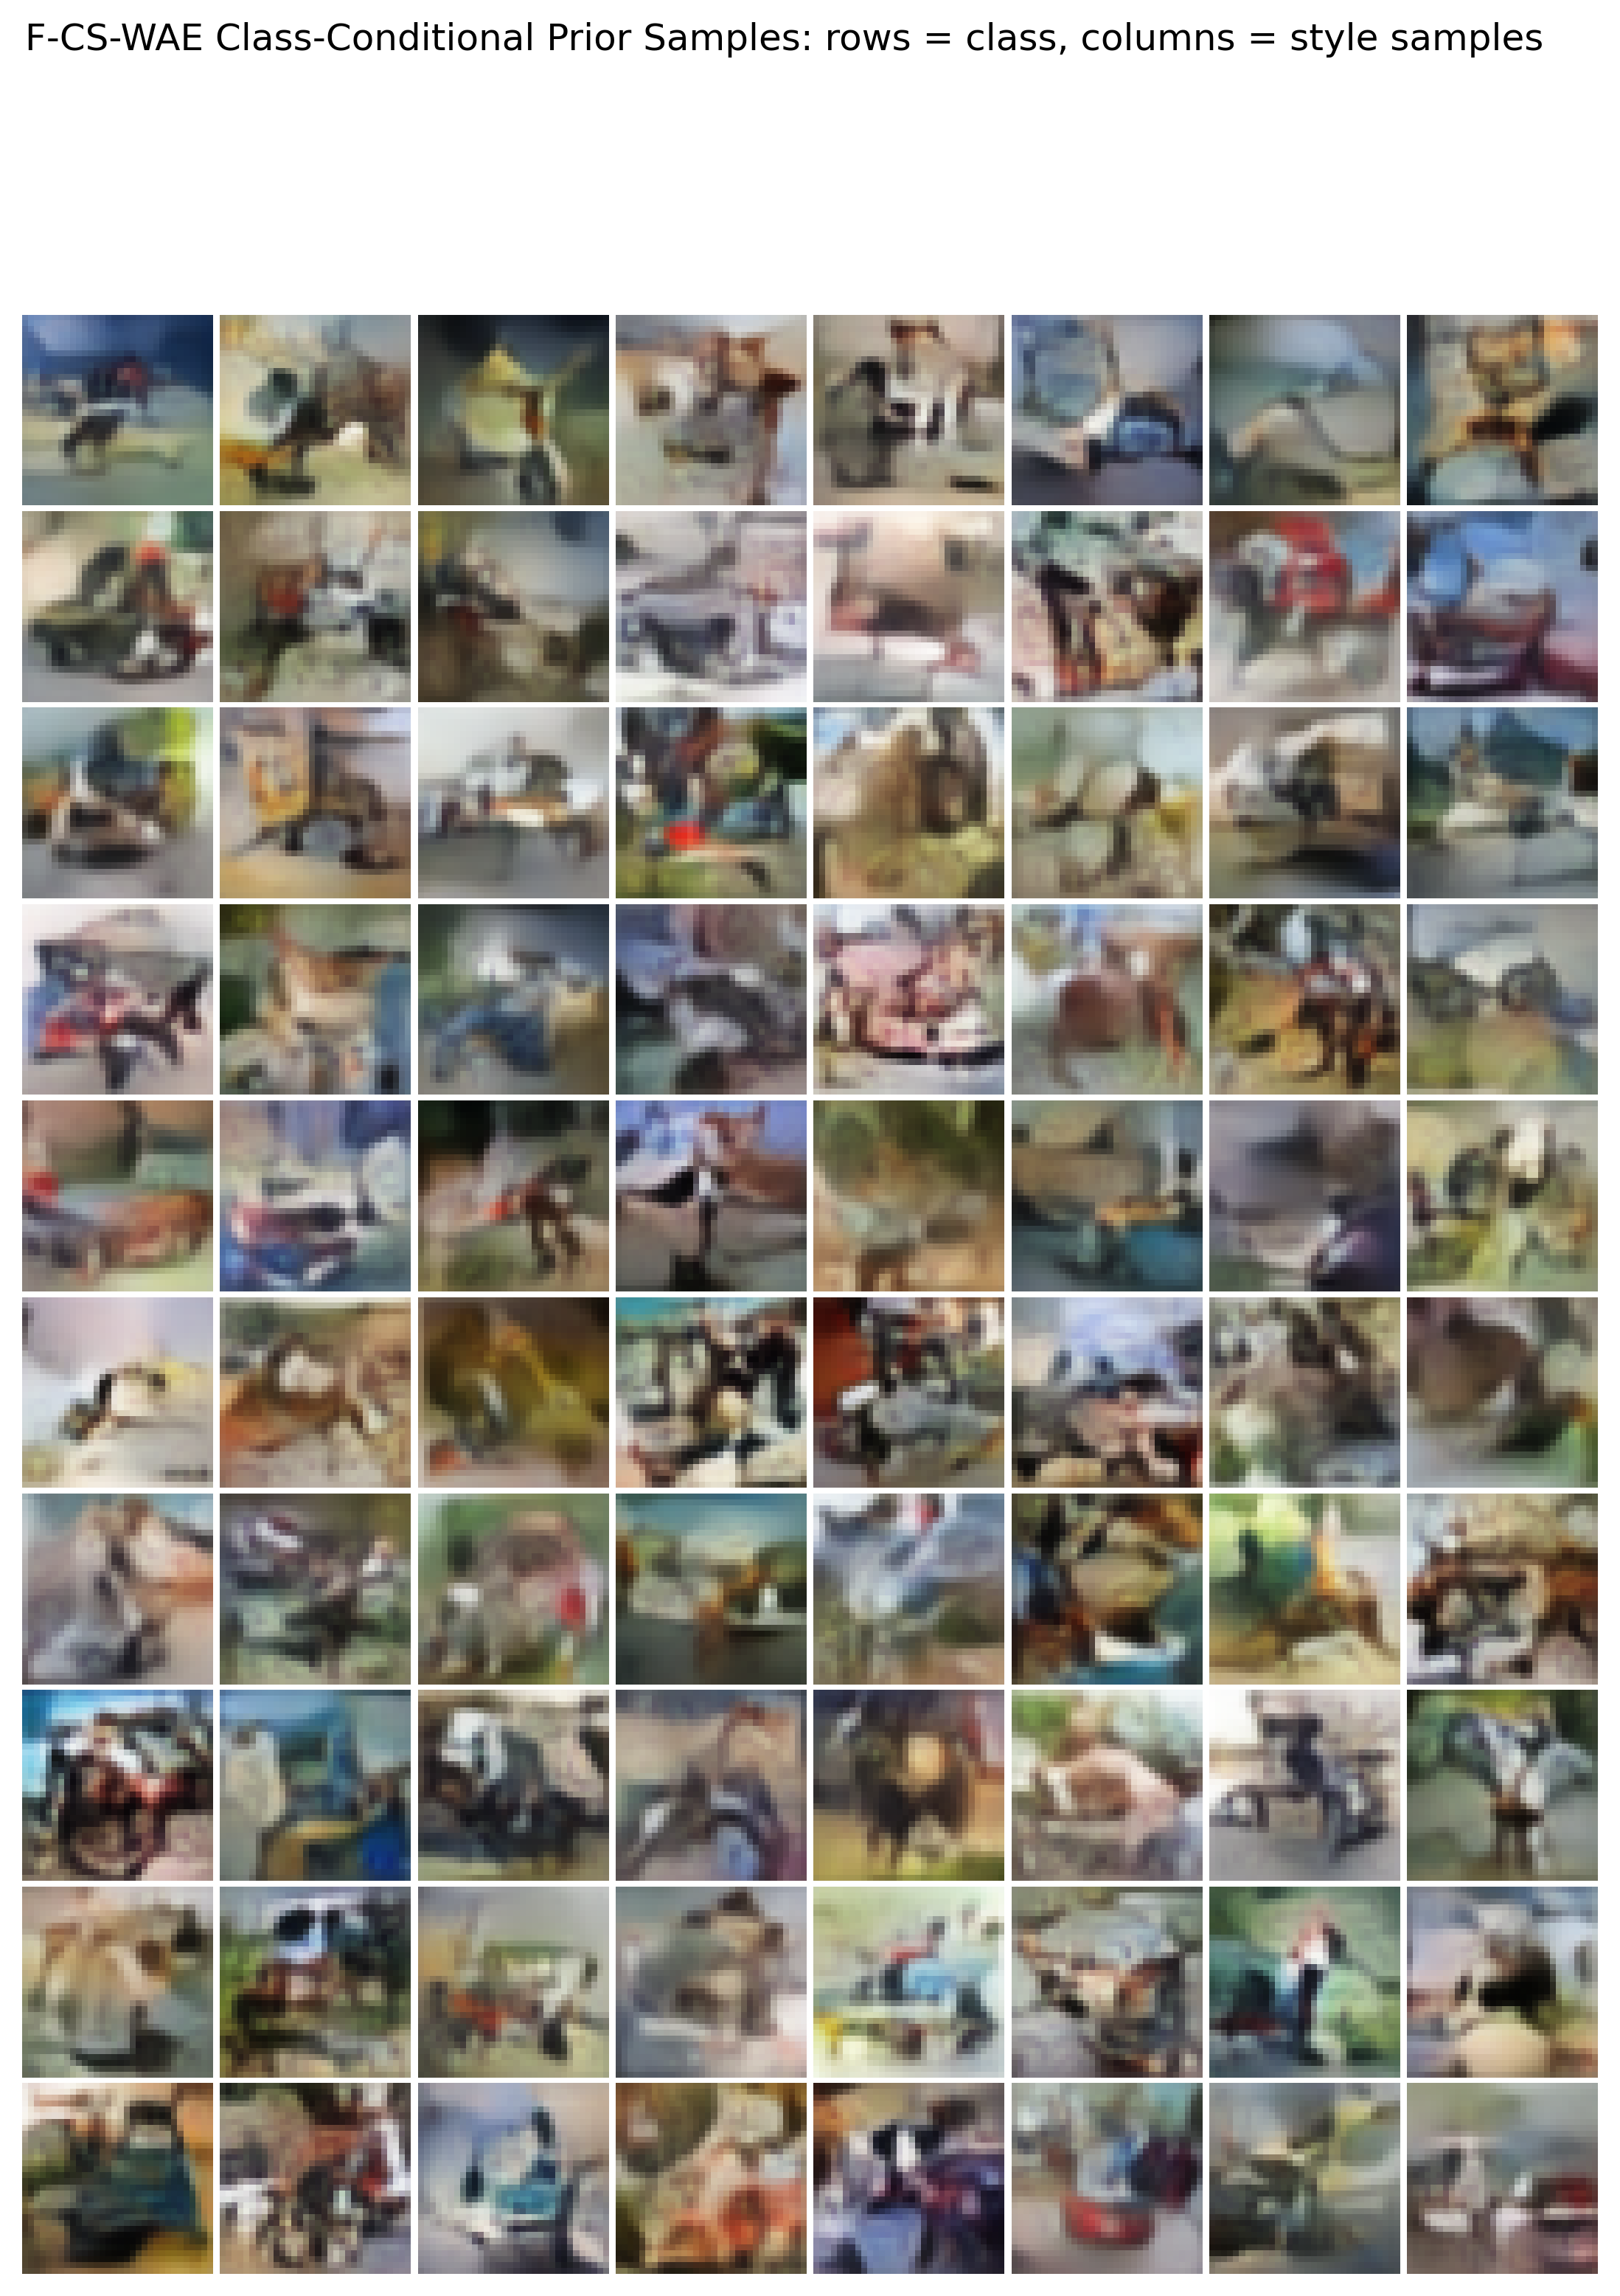
\includegraphics[width=0.95\linewidth]{cifar10_class_prior_grid.png}
\caption{CIFAR-10 class-conditional prior samples.
         Each row corresponds to one class prior ($\zs\sim\mathcal{N}(0,I)$).}
\label{fig:cifar-samples}
\end{figure}

\begin{figure}[t]
\centering
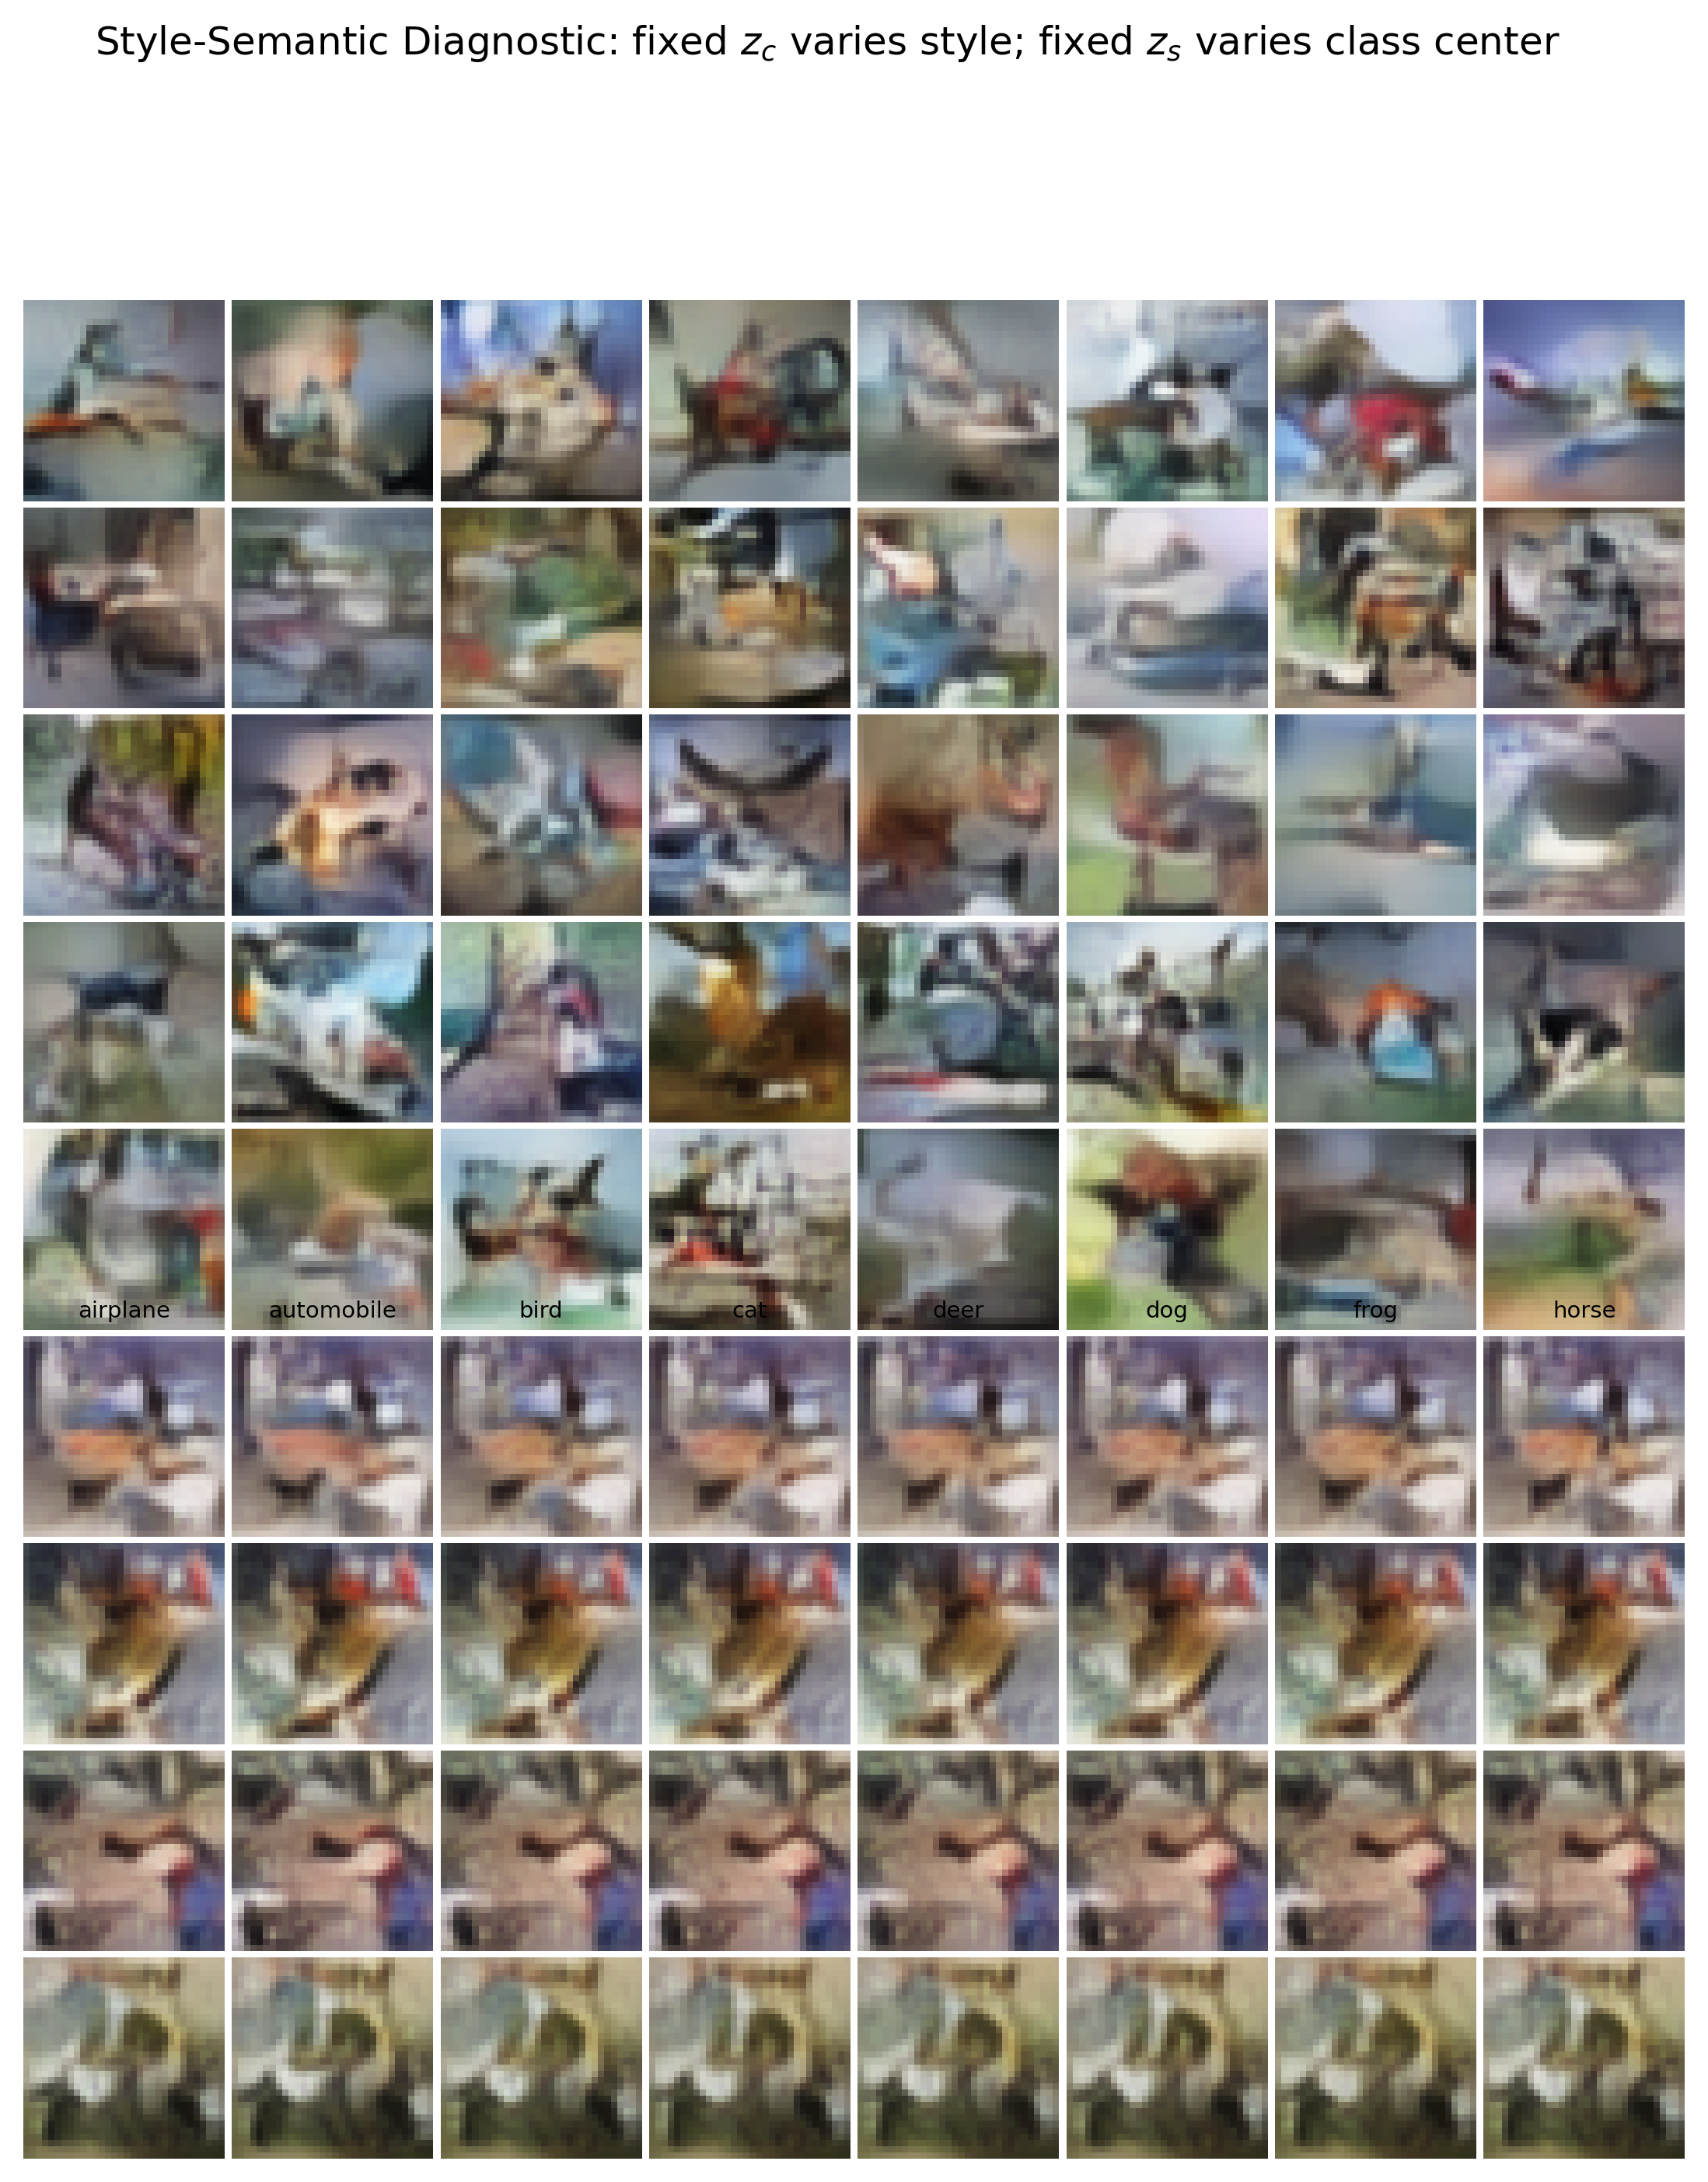
\includegraphics[width=0.95\linewidth]{cifar10_style_semantic_grid.png}
\caption{CIFAR-10 factorization probe.
         \emph{Columns:} fixed $\zc$, varying $\zs$.
         \emph{Rows:} fixed $\zs$, varying $\zc$.
         Style modulates texture and color; semantics modulate coarse class identity.}
\label{fig:cifar-style}
\end{figure}

Figure~\ref{fig:cifar-training} shows training curves across seeds, confirming that
the four-phase schedule keeps all loss terms stable after each transition.

\begin{figure}[t]
\centering
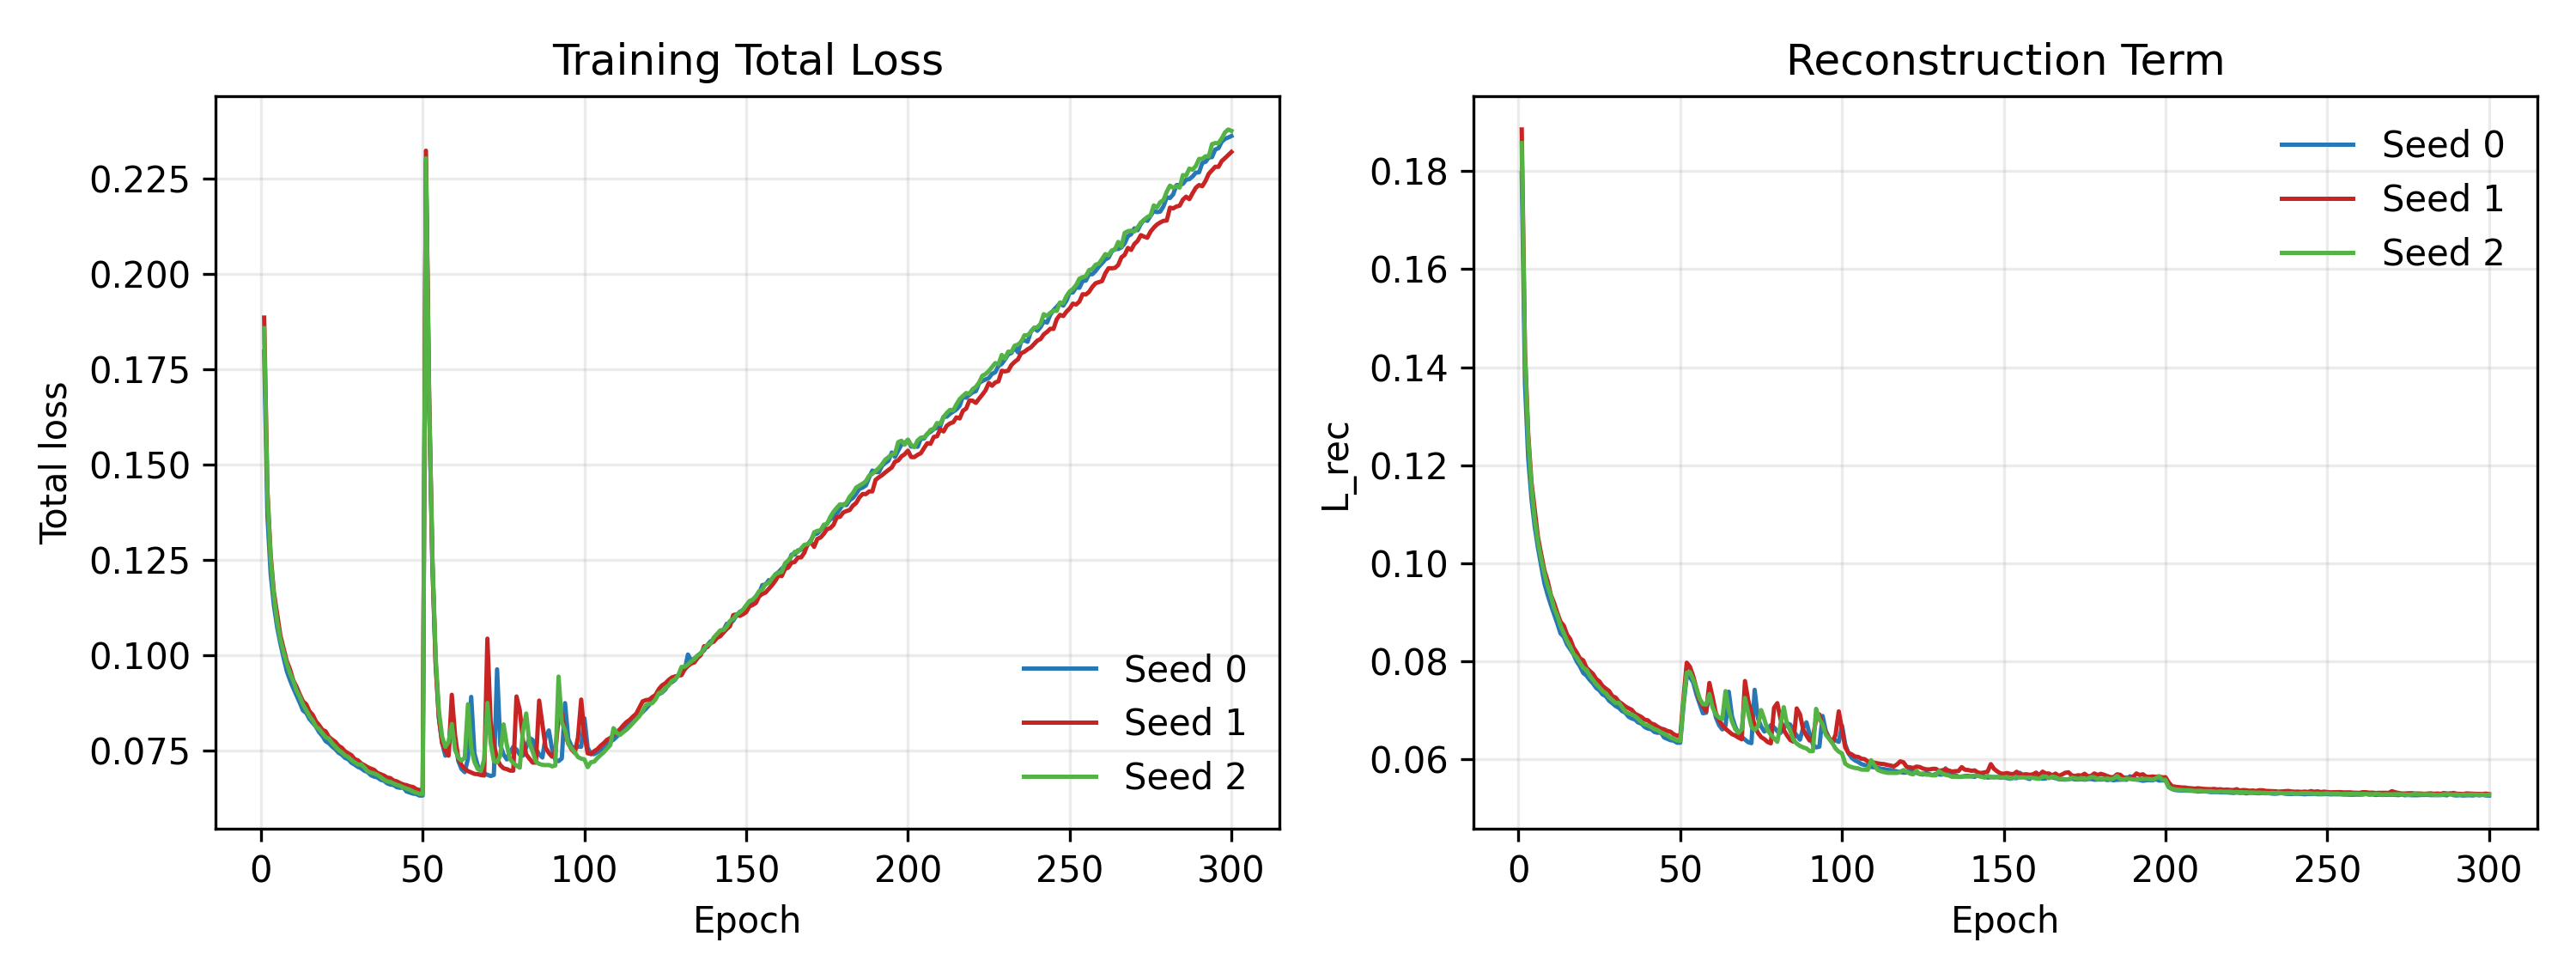
\includegraphics[width=0.95\linewidth]{cifar10_training_curves.png}
\caption{CIFAR-10 training curves. Phase transitions (epochs 50, 100, 200) are
         visible as step-changes; all terms converge smoothly.}
\label{fig:cifar-training}
\end{figure}

\subsection{MNIST: Strong Clustering, Surprising Generation Failure}
\label{sec:mnist}

Table~\ref{tab:mnist} compares \ours{} (seed 0) to the single-latent \simple{}
(seed 0) on MNIST.
\ours{} strongly improves clustering ($+11.8$ ACC points) and reconstruction
(SSIM $0.983$ vs $0.813$, PSNR $26.88$ vs $16.38$~dB).
However, \ours{} FID is $73.99$ while \simple{} FID is $26.95$: prior samples from
the single-latent model look like plausible digits; \ours{} prior samples are often
shapeless or decode as the wrong class.

\begin{table}[t]
\centering
\caption{MNIST seed-0 comparison.
         \simple{}: single-latent Spherical Cauchy WAE.
         \todo{Expand to 3 seeds and report mean$\pm$std for both models.}}
\label{tab:mnist}
\begin{tabular}{lrrrrrrr}
\toprule
Method & ACC & NMI & ARI & SSIM & PSNR & LPIPS & FID \\
\midrule
\simple{}        & 0.8735 & 0.8863 & 0.8411 & 0.8127 & 16.38 & 0.0603 & \textbf{26.95} \\
\textbf{\ours{}} & \textbf{0.9915} & \textbf{0.9758} & \textbf{0.9813}
                 & \textbf{0.9833} & \textbf{26.88} & \textbf{0.0120} & 73.99 \\
\bottomrule
\end{tabular}
\end{table}

This result illustrates a critical warning for generative clustering: excellent
reconstruction and clustering can coexist with poor prior sampling.
Reporting only ACC/NMI/ARI would overstate the model's generative quality.

\subsection{Failure Diagnosis: Conditional Style Mismatch}
\label{sec:diagnosis}

We probe the MNIST \ours{} checkpoint by encoding 2{,}048 test images and analyzing
the style latent $\zs$.

\paragraph{Marginal statistics (look healthy).}
Per-dimension variance $\approx 0.973$;
multi-scale MMD to $\mathcal{N}(0,I)$ $\approx 0.0017$.
By the aggregate marginal test, style regularization appears to have succeeded.

\paragraph{Conditional statistics (reveal the problem).}
Class-conditional style means are far apart:
average pairwise $\ell_2$ distance between the 10 class style means $\approx 6.25$,
while within-class style norm $\approx 10.25$.
The class-to-within ratio is not small---style codes carry strong class information
despite the marginal being well-matched.

\paragraph{Causal mechanism.}
During training the decoder sees $(\zc,\zs)$ pairs from the \emph{same} image.
Both variables encode the same class, so the decoder can learn class-specific
interactions between them.
At generation time, $\zc$ encodes class $k$ but $\zs\sim\mathcal{N}(0,I)$ is an
average over all classes.
The decoder encounters a cross-class pair that never occurred in training and
produces an inconsistent image.

\paragraph{Formal statement.}
Global style MMD enforces:
\begin{equation}
  q(\zs) = \mathbb{E}_y[q(\zs\mid y)] \approx \mathcal{N}(0,I),
\end{equation}
but this does not imply $q(\zs\mid y{=}k)\approx\mathcal{N}(0,I)$ for any individual
class $k$, nor does it imply $\zs\perp y$.
Matching the marginal is necessary but not sufficient for class-independent generation.
This is a structural failure mode for any factorized WAE using only a global style
regularizer.

Figure~\ref{fig:style-diagnostic} visualizes the class-conditional style structure.

\begin{figure}[t]
\centering
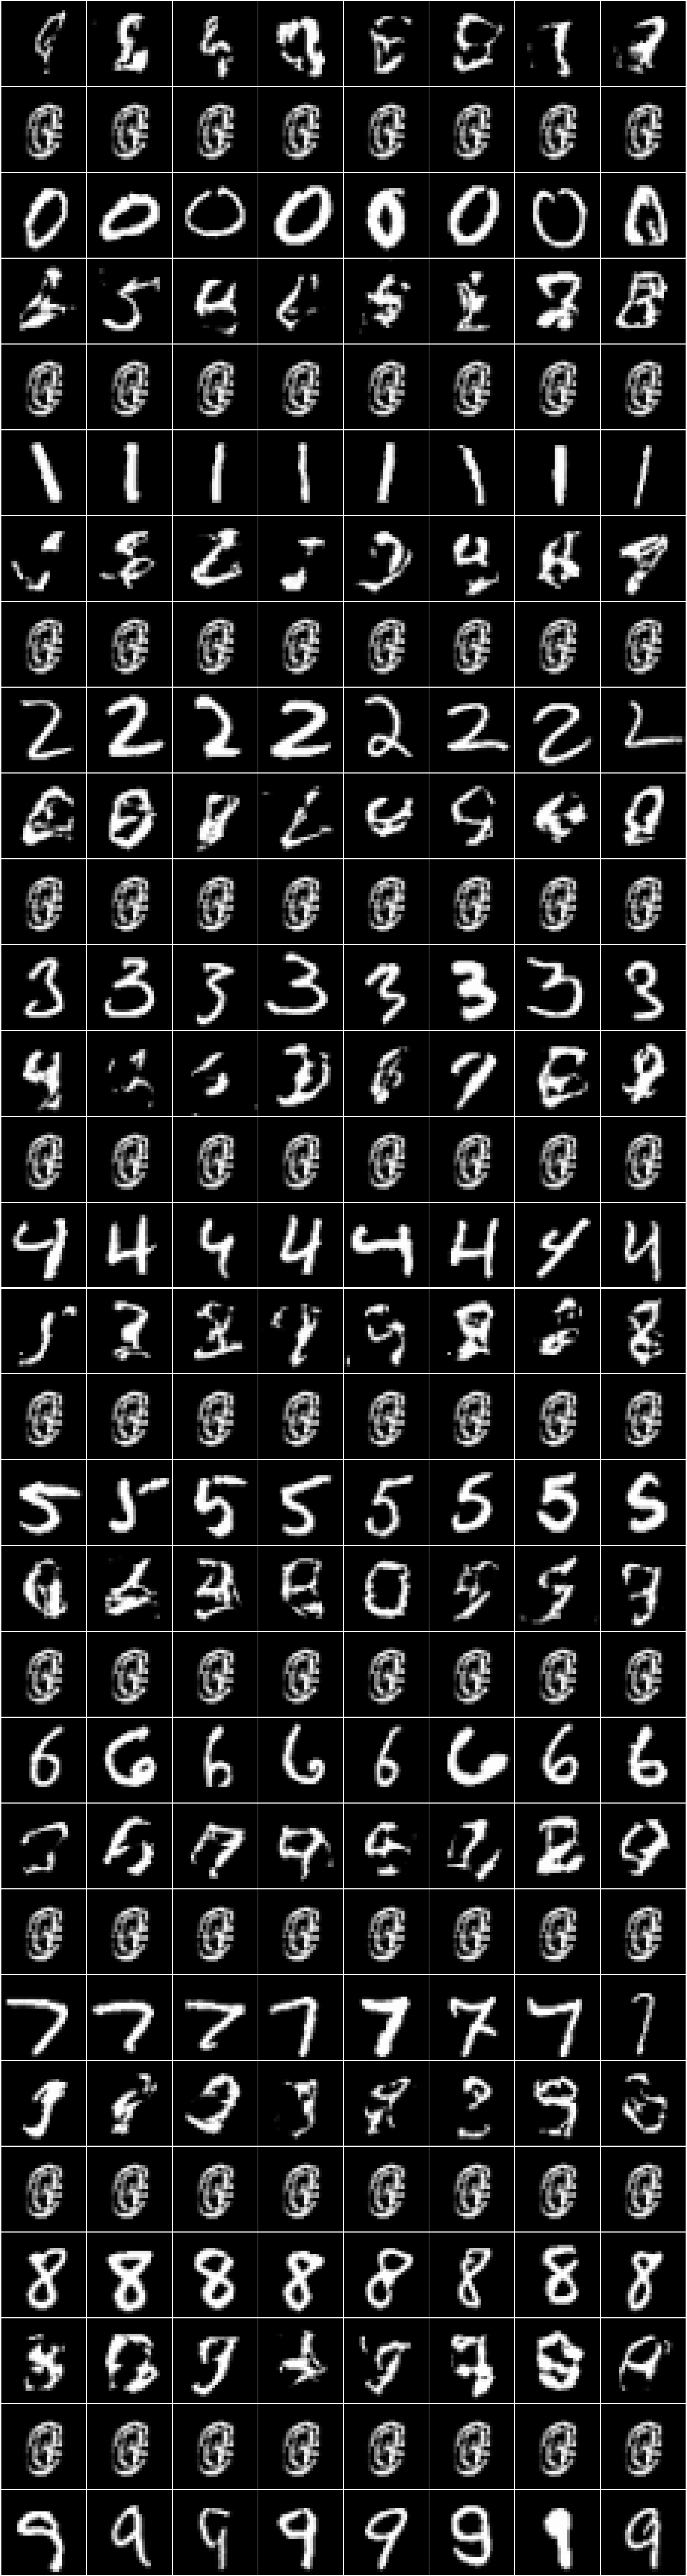
\includegraphics[width=0.88\linewidth]{mnist_style_prior_diagnostic.png}
\caption{MNIST style latent diagnostic.
         Despite global MMD $\approx 0.0017$, class-conditional style means
         are clearly separated, confirming that $\zs\not\perp y$.}
\label{fig:style-diagnostic}
\end{figure}

\subsection{Representation-Aware Sampling}
\label{sec:sampling}

We evaluate four style sampling strategies on the trained MNIST checkpoint.
For each strategy, 10 images per class are generated, re-encoded through the trained
\ours{} auxiliary classifier, and the fraction decoded as the intended class
is reported as \emph{self-accuracy}.
Pixel diversity (mean per-pixel standard deviation) is also reported.

\begin{table}[t]
\centering
\caption{MNIST generation under representation-aware style sampling strategies.
         Self-ACC: fraction of generated images classified as the intended class
         by the trained \ours{} classifier.
         All strategies sample $\zc$ from the Spherical Cauchy class prior.}
\label{tab:sampling}
\begin{tabular}{lrrr}
\toprule
Style sampling $\zs$ & Self-ACC $\uparrow$ & Confidence $\uparrow$ & Diversity $\uparrow$ \\
\midrule
Global Gaussian $\mathcal{N}(0,I)$           & 0.15 & 0.934 & 0.151 \\
Class mean $\bar\mus^{(k)}$                  & 1.00 & 1.000 & 0.132 \\
Class diagonal Gaussian, $\tau=0.50$         & 1.00 & 0.990 & 0.139 \\
Class diagonal Gaussian, $\tau=0.25$         & \textbf{1.00} & \textbf{1.000} & 0.135 \\
Empirical style bank                         & 1.00 & 1.000 & \textbf{0.182} \\
\bottomrule
\end{tabular}
\end{table}

Table~\ref{tab:sampling} makes four points clear.
First, the global Gaussian sampler fails catastrophically ($15\%$), confirming the
diagnosis.
Second, any conditioning on class restores perfect self-accuracy ($100\%$).
Third, the class mean style collapses within-class diversity (lowest diversity score).
Fourth, the empirical style bank (oracle that reuses encoded training styles) achieves
the highest diversity but requires training data at generation time.
The class-conditional diagonal Gaussian with $\tau=0.25$ is the recommended
generation prior: it is a true parametric sampler, gives perfect class consistency,
and preserves more variation than a point estimate.

Figure~\ref{fig:sampling-strategies} shows generated images under each strategy.

\begin{figure*}[t]
\centering
\begin{subfigure}[t]{0.24\linewidth}
  \centering
  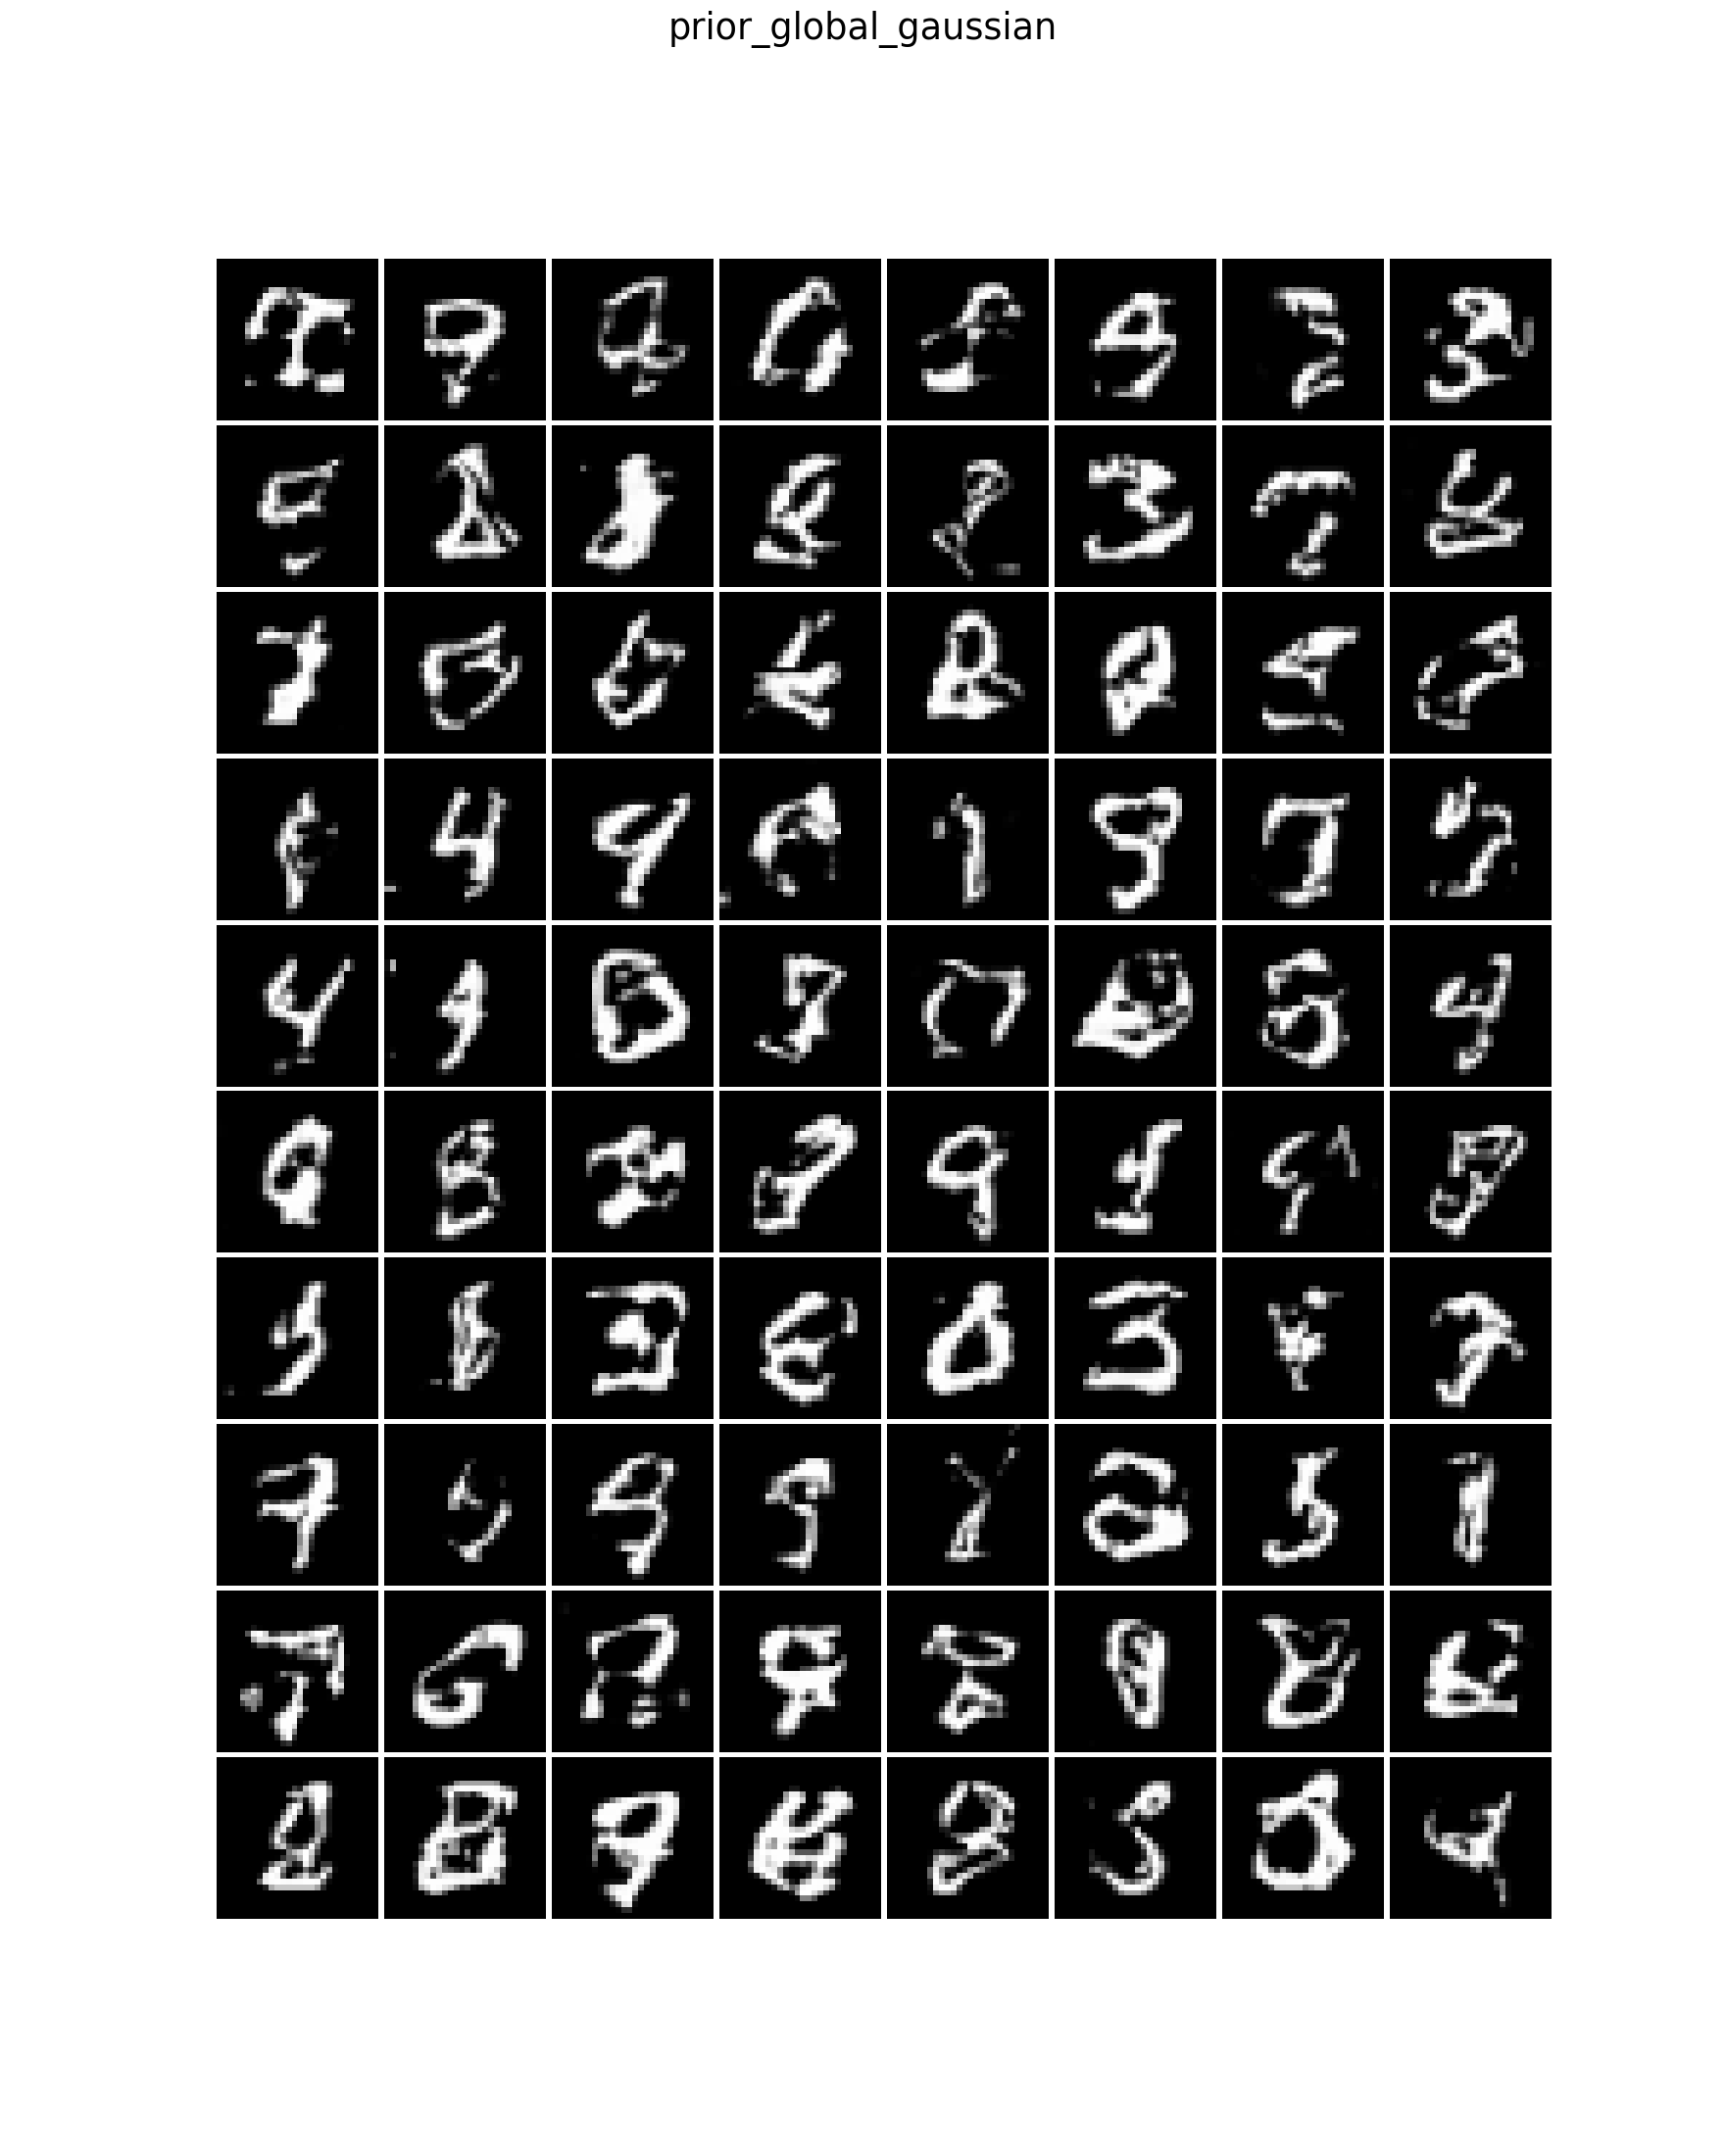
\includegraphics[width=\linewidth]{mnist_sampling_global_gaussian.png}
  \caption{Global Gaussian\\(self-ACC: 15\%)}
\end{subfigure}
\hfill
\begin{subfigure}[t]{0.24\linewidth}
  \centering
  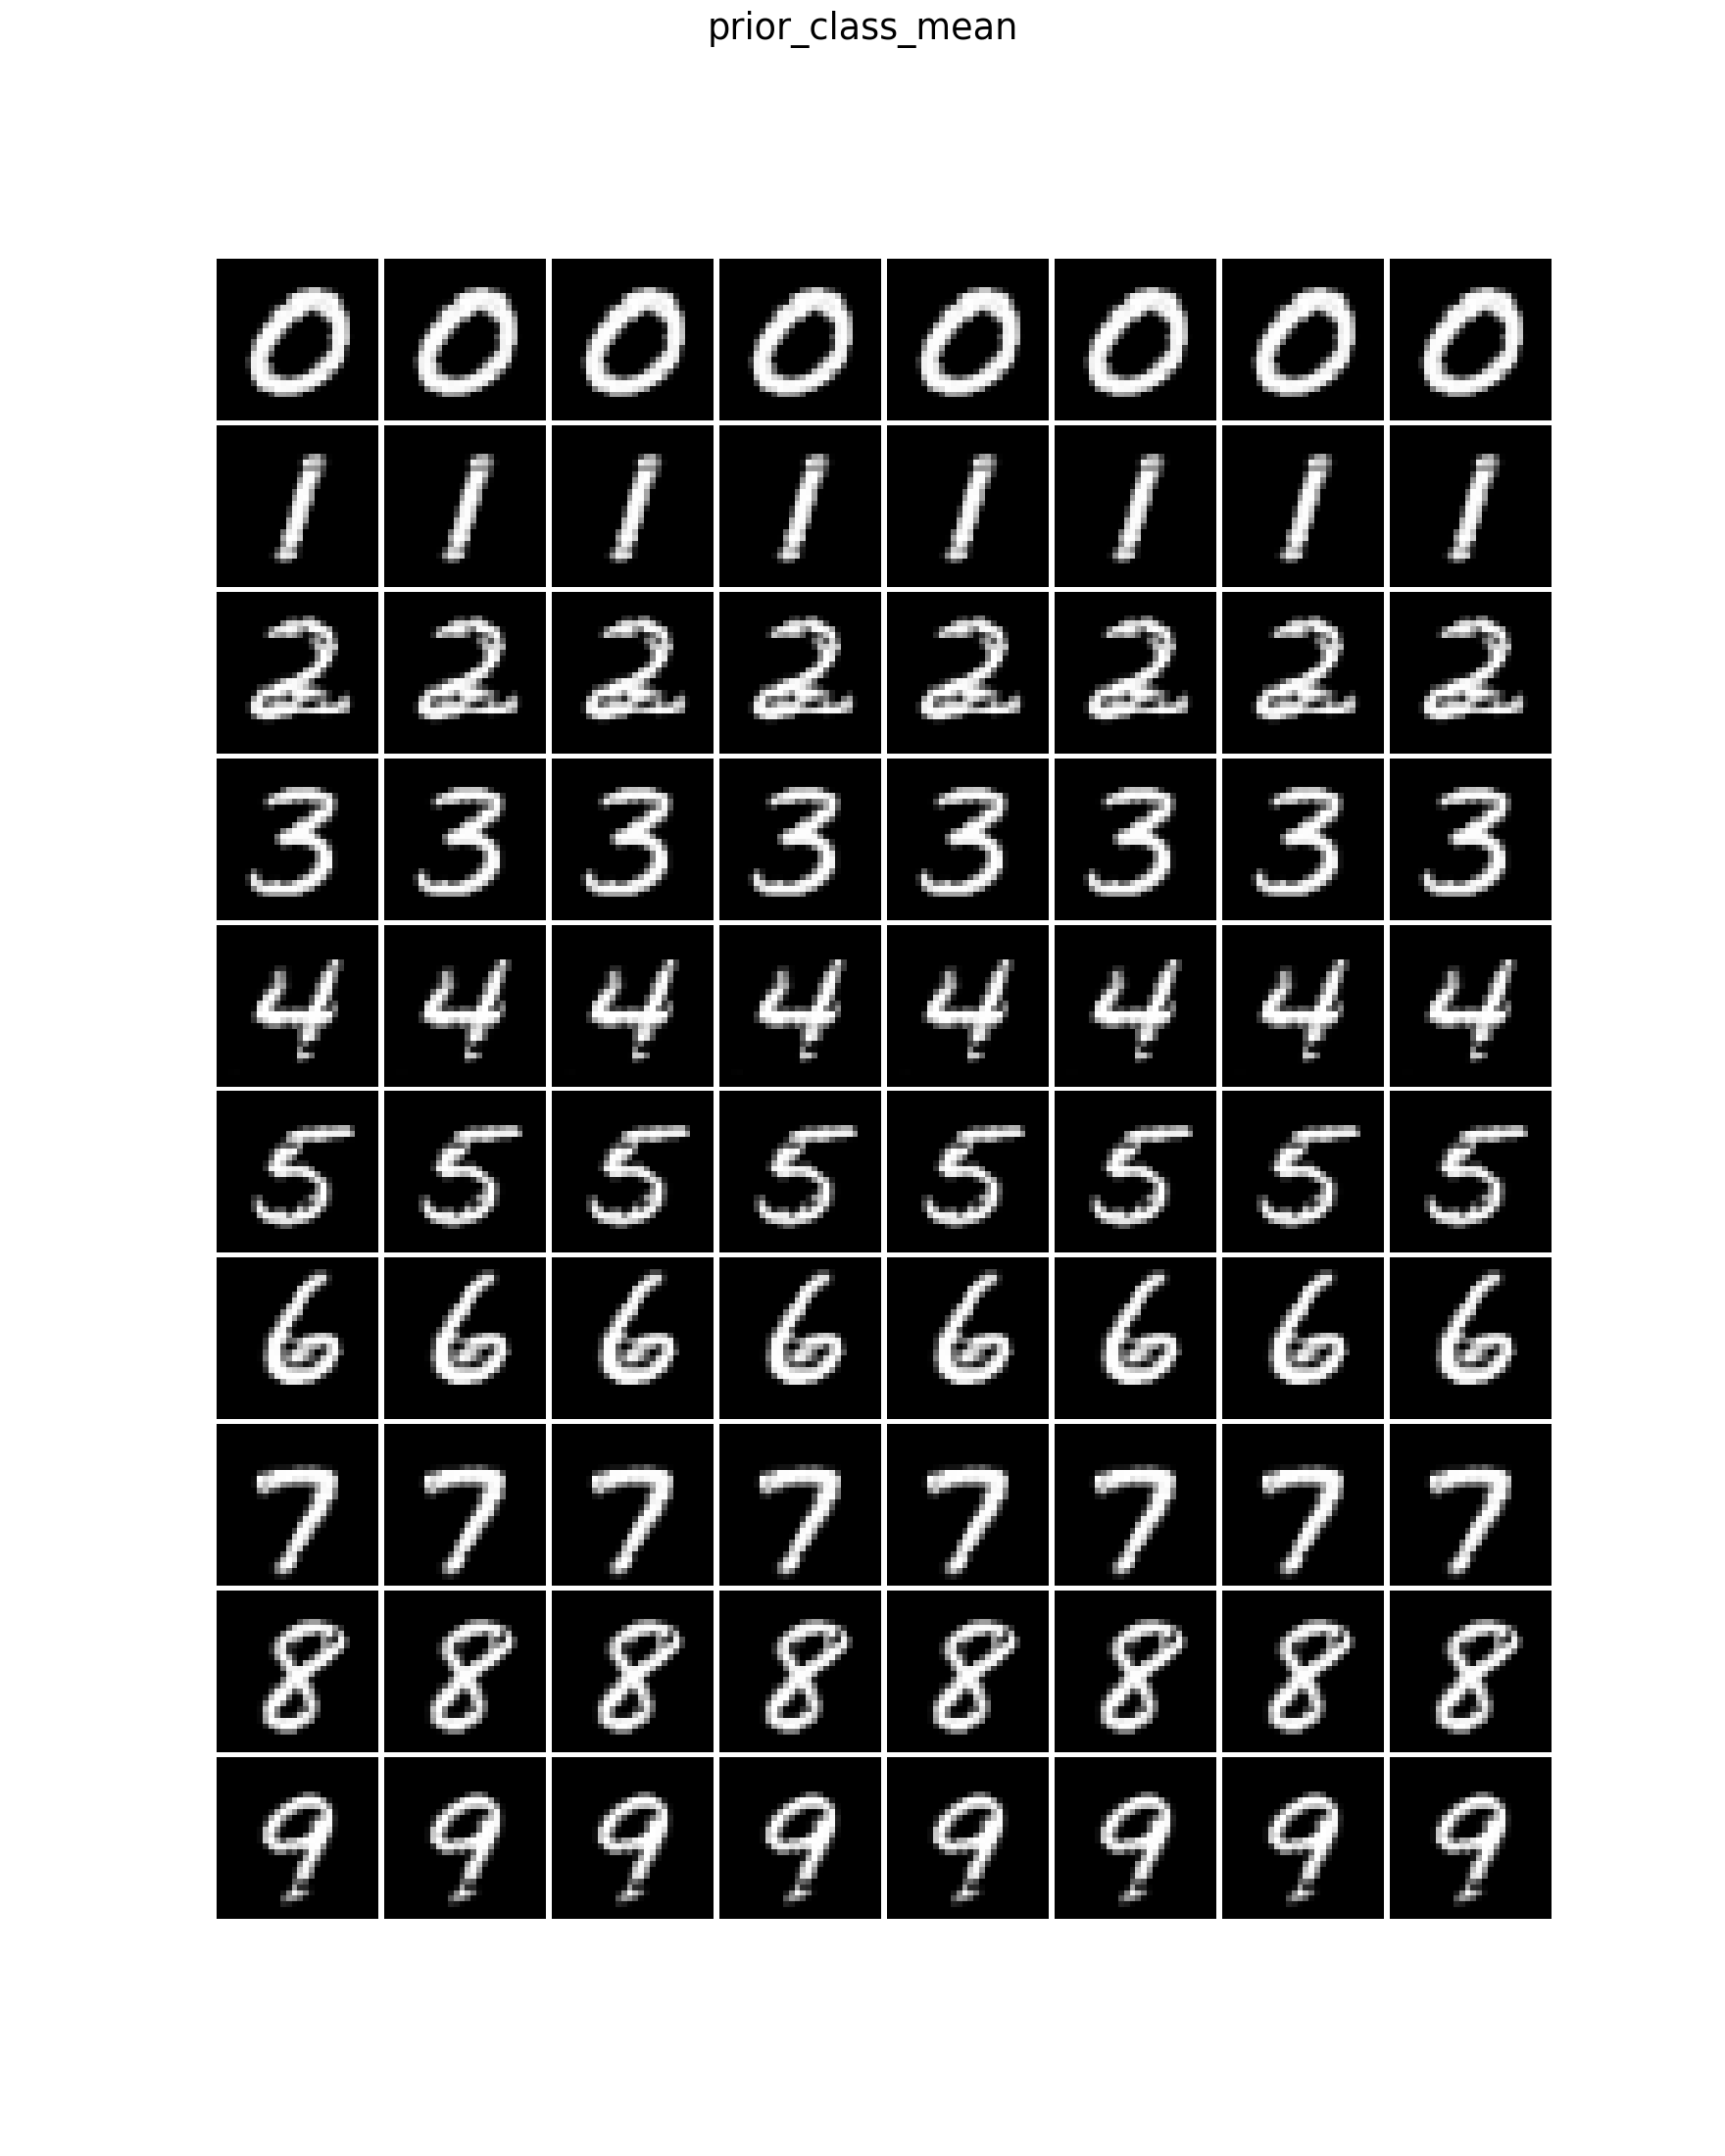
\includegraphics[width=\linewidth]{mnist_sampling_class_mean.png}
  \caption{Class mean style\\(self-ACC: 100\%)}
\end{subfigure}
\hfill
\begin{subfigure}[t]{0.24\linewidth}
  \centering
  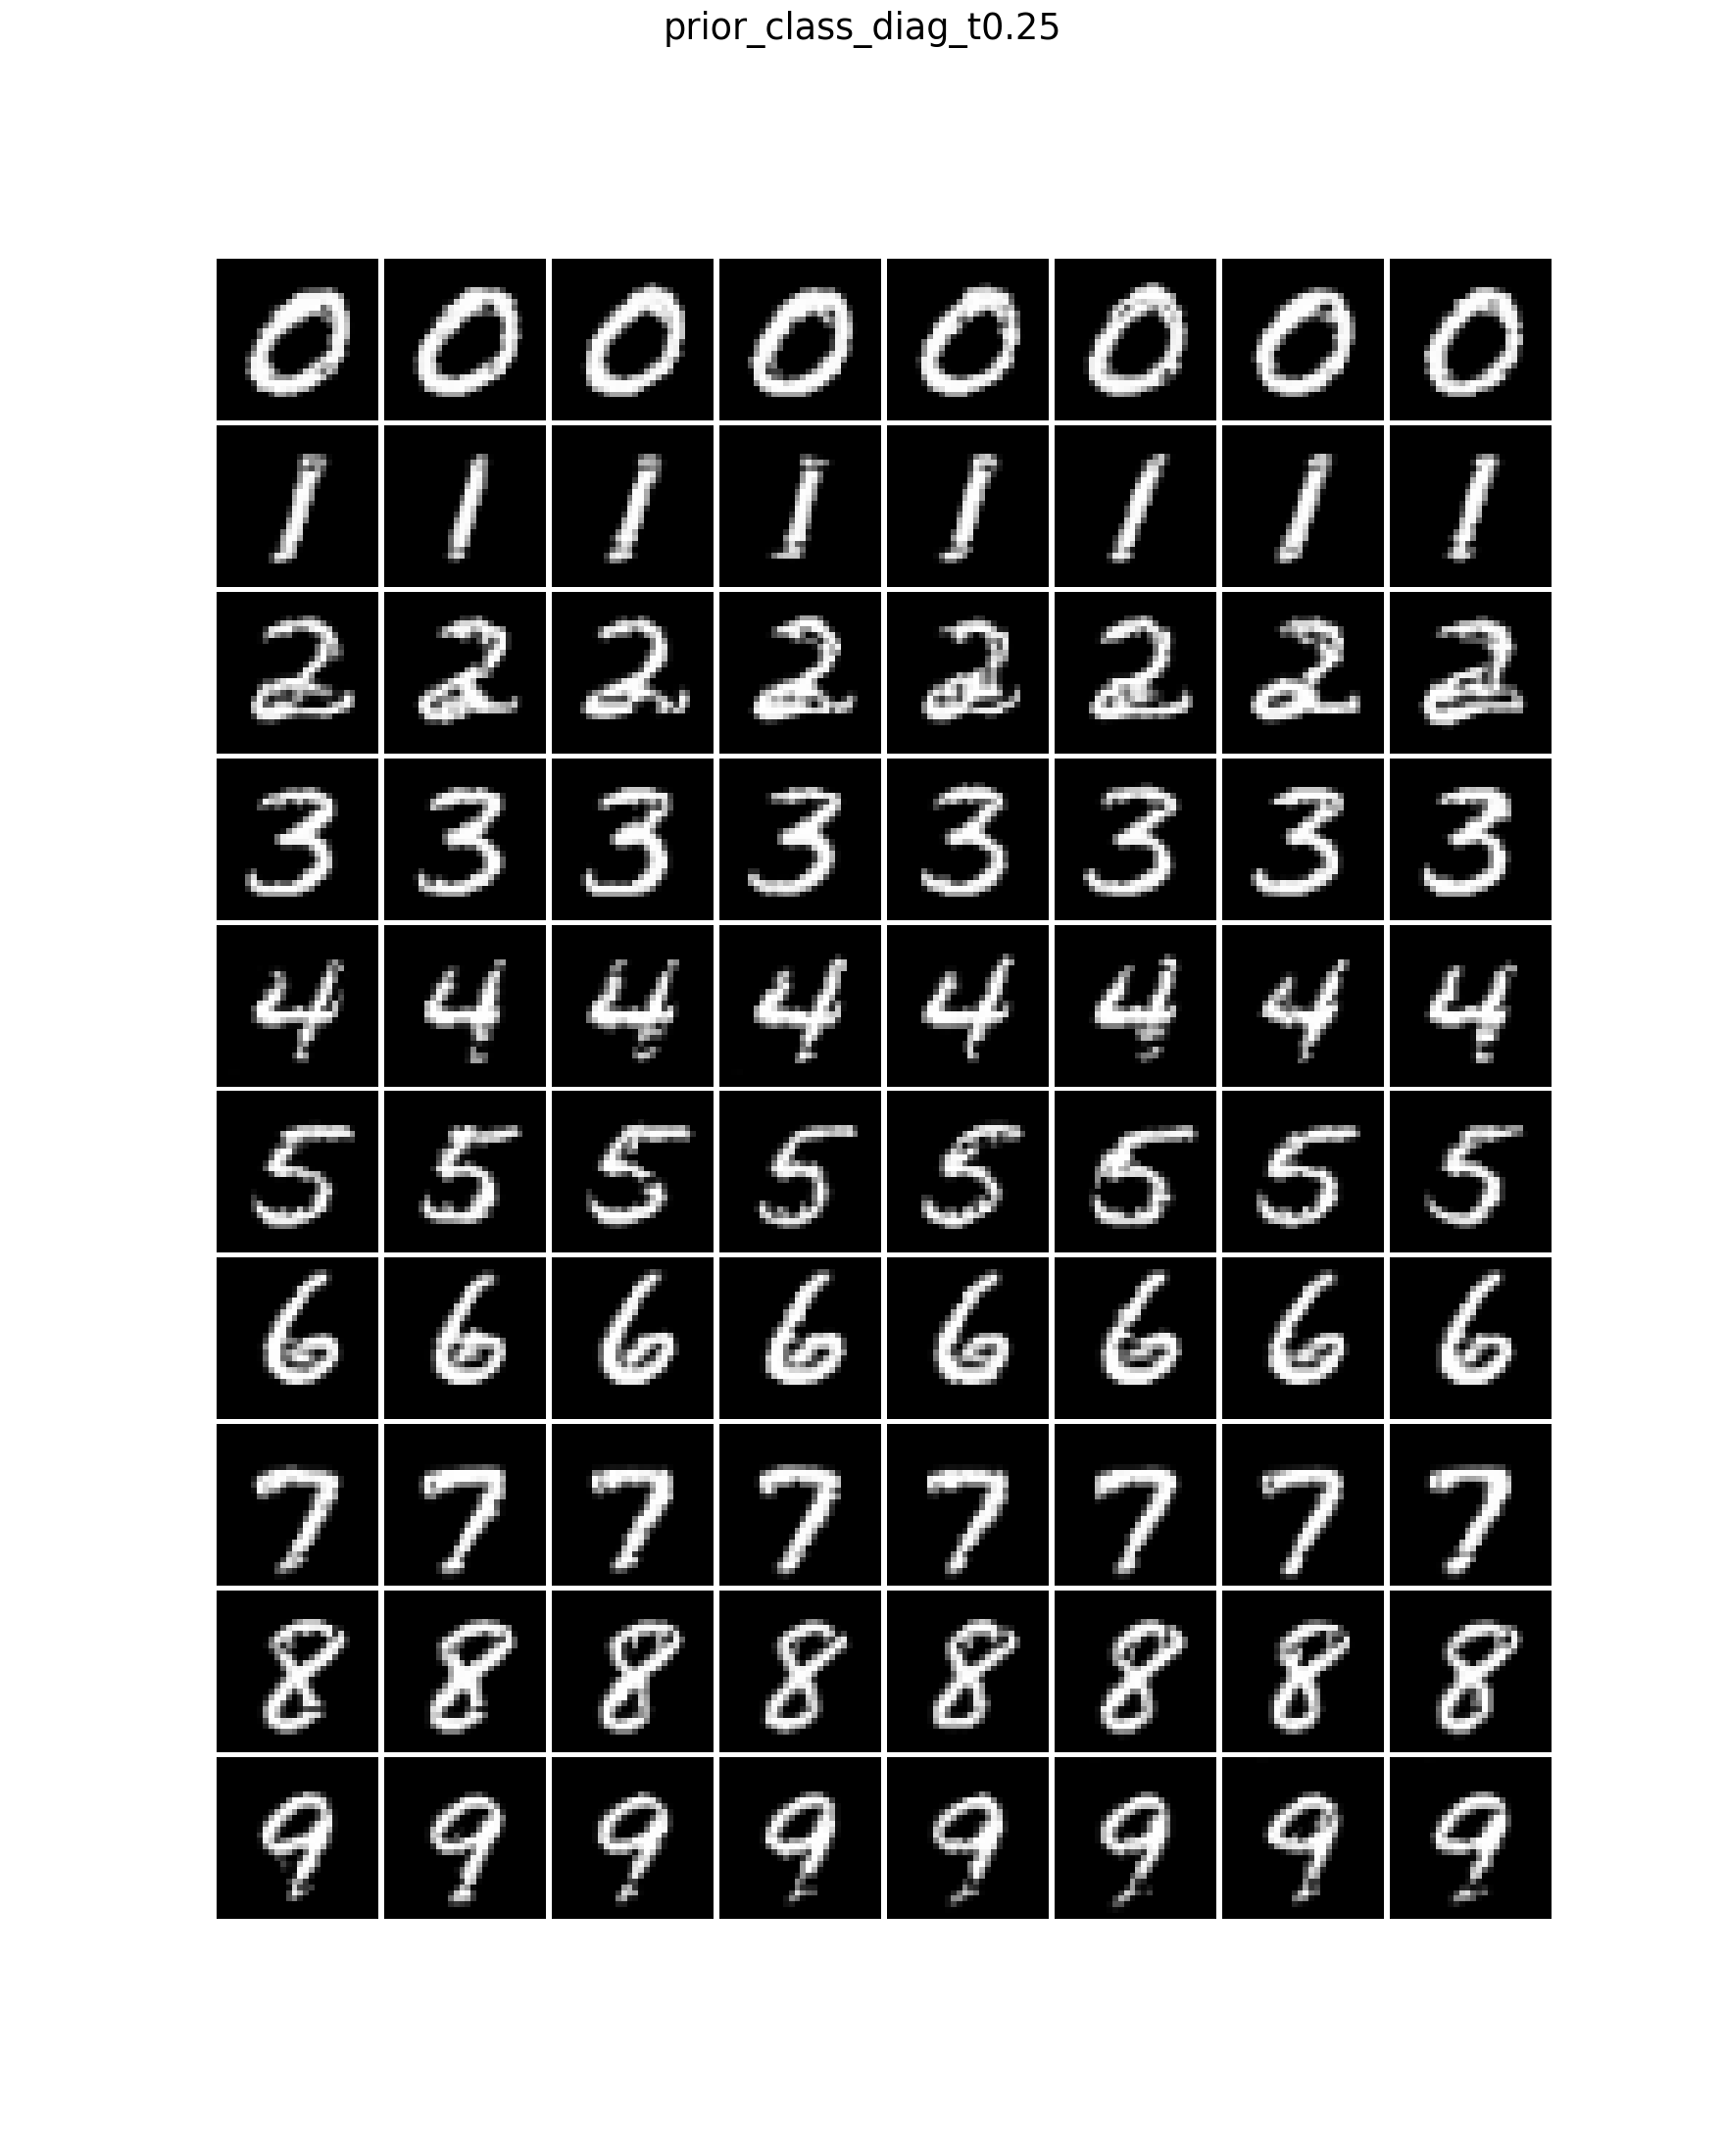
\includegraphics[width=\linewidth]{mnist_sampling_class_diag_t025.png}
  \caption{Class diag., $\tau{=}0.25$\\(self-ACC: 100\%)}
\end{subfigure}
\hfill
\begin{subfigure}[t]{0.24\linewidth}
  \centering
  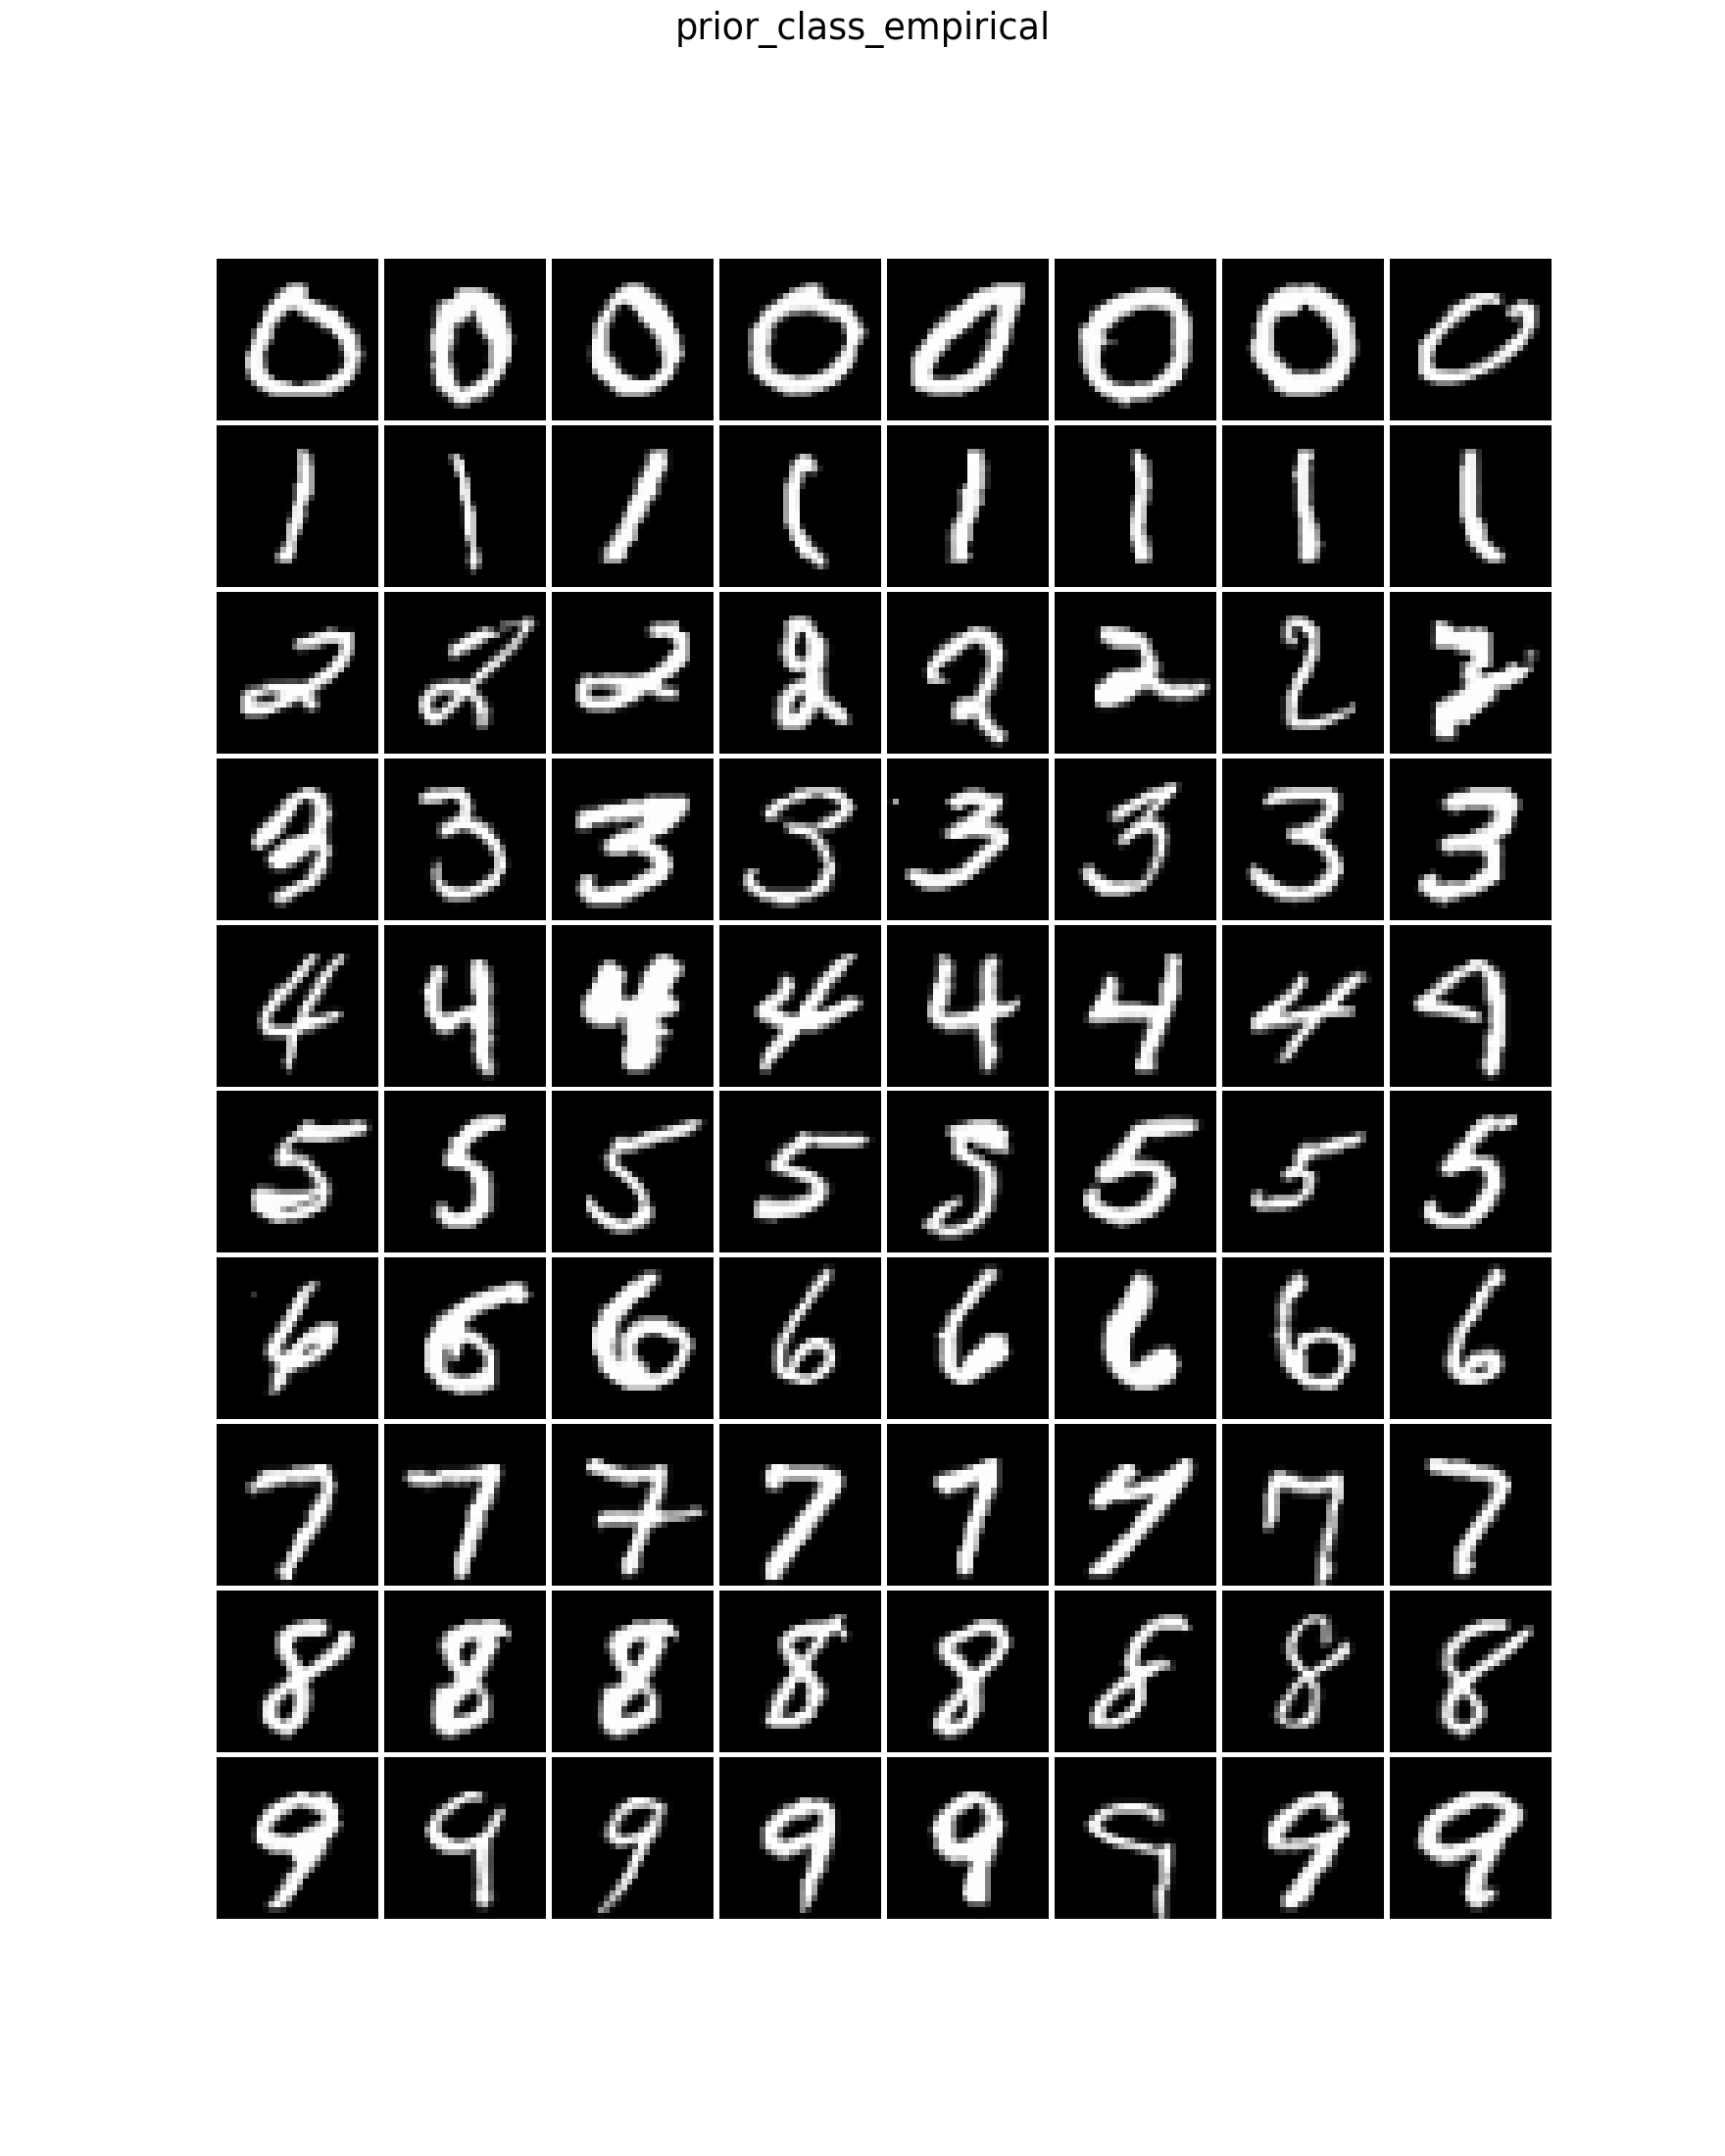
\includegraphics[width=\linewidth]{mnist_sampling_class_empirical.png}
  \caption{Empirical style bank\\(self-ACC: 100\%)}
\end{subfigure}
\caption{MNIST generation under representation-aware style sampling.
         Global Gaussian sampling produces shapeless images;
         all class-conditional strategies restore correct digit identity.
         Class diagonal Gaussian ($\tau=0.25$) gives the best balance of
         class consistency and intra-class diversity.}
\label{fig:sampling-strategies}
\end{figure*}

\subsection{Ablation Study}
\label{sec:ablations}

Table~\ref{tab:ablations} reports CIFAR-10 clustering results for key design
choices.
The most informative comparisons are discussed below.

\begin{table}[t]
\centering
\caption{CIFAR-10 ablations, seed 0.
         \todo{Run all ablation variants and fill in numbers.}}
\label{tab:ablations}
\renewcommand{\arraystretch}{1.05}
\begin{tabular}{lccc}
\toprule
Variant & ACC & NMI & ARI \\
\midrule
\ours{} (full, seed 0)       & 0.8149 & 0.6622 & 0.6438 \\
\midrule
\emph{Remove components:}    & & & \\
\quad No $\zs$ (semantic-only)            & \todo{} & \todo{} & \todo{} \\
\quad No class MMD ($\alpha{=}0$)         & \todo{} & \todo{} & \todo{} \\
\quad No aggregated MMD ($\beta{=}0$)     & \todo{} & \todo{} & \todo{} \\
\quad No style MMD ($\gamma{=}0$)         & \todo{} & \todo{} & \todo{} \\
\quad No auxiliary classifier ($\eta{=}0$)& \todo{} & \todo{} & \todo{} \\
\midrule
\emph{Prior geometry:}       & & & \\
\quad Gaussian semantic prior             & \todo{} & \todo{} & \todo{} \\
\quad vMF semantic prior                  & \todo{} & \todo{} & \todo{} \\
\midrule
\emph{Proposed extension:}   & & & \\
\quad + Per-class style MMD ($\delta{>}0$)& \todo{} & \todo{} & \todo{} \\
\bottomrule
\end{tabular}
\end{table}

\textbf{No $\zs$ (semantic-only).}
Removing the style variable tests whether $\zc$ alone is sufficient.
On simpler datasets (MNIST, Fashion-MNIST) we expect this to perform competitively
because class identity explains most visual variation.
On CIFAR-10, the full model is expected to be superior because $\zs$ absorbs
intra-class variation that would otherwise corrupt $\zc$.

\textbf{No class MMD.}
Removing $\mathcal{L}_{\mathrm{class}}$ collapses supervised prior alignment and
is expected to drastically reduce clustering accuracy, since class-conditional
structure in $\zc$ comes primarily from this term.

\textbf{Prior geometry.}
Replacing the Spherical Cauchy prior with a Gaussian (Euclidean semantic)
or von Mises-Fisher tests whether hyperspherical geometry and the heavy-tailed
Spherical Cauchy prior are both necessary.

\textbf{Per-class style MMD.}
Adding $\mathcal{L}_{\mathrm{style\text{-}cls}}$ should not reduce clustering quality
but should fix the generation failure: prior samples with $\zs\sim\mathcal{N}(0,I)$
should become reliable.
\todo{Re-evaluate FID with global Gaussian sampling after training with per-class
style MMD and report in the final ablation table.}

% ============================================================
\section{Discussion}
% ============================================================

\paragraph{Why CIFAR-10 and MNIST differ.}
On CIFAR-10, naive prior sampling ($\zs\sim\mathcal{N}(0,I)$) yields FID $83.04$
and visually plausible images.
We hypothesize that high intra-class visual diversity on CIFAR-10 (pose, color,
background, texture) causes $\zs$ to carry relatively more semantically neutral
variation, weakening class-conditional style dependence.
On MNIST, classes are more uniform: intra-class appearance is nearly constant,
so the decoder relies heavily on class information in $\zs$, amplifying the
conditional mismatch.
This predicts that per-class style MMD will matter more for simpler,
more class-uniform datasets.

\paragraph{Global vs.\ conditional regularization.}
Global aggregate matching is a standard design choice in WAEs and
disentanglement models~\citep{tolstikhin2017wasserstein,kim2018disentangling}.
Our results show it is insufficient when the style variable must be class-invariant
for generation.
Per-class style MMD can be seen as a supervised version of total correlation
penalties: rather than penalizing all pairwise dependencies among factors, it
directly penalizes the single dependency $\zs\not\perp y$ that causes generation
failure.
A complementary approach is an HSIC-style penalty or gradient-reversal classifier
on $(\zs,y)$, which would not require class-stratified batching.

\paragraph{The reconstruction--generation gap.}
The MNIST \ours{} checkpoint achieves SSIM $0.983$ and PSNR $26.88$~dB yet has
FID $73.99$ for naive prior sampling.
This confirms a well-known but often ignored lesson: reconstruction quality measures
fidelity on the posterior manifold, not on the prior.
A decoder can achieve near-perfect reconstruction on encoded inputs while being
unreliable for samples from the intended prior.
Evaluation of generative clustering models should always include both reconstruction
\emph{and} generation metrics; reporting only ACC/NMI/ARI and SSIM/PSNR can
completely hide this failure.

\paragraph{Generality of the finding.}
The conditional style mismatch failure is not specific to \ours.
Any factorized generative model (including $\beta$-TCVAE variants, conditional WAEs,
or similar architectures) that uses a global aggregate regularizer on a style-like
variable should verify that the variable has not become class-dependent before
claiming class-conditional generation quality.
The diagnostic we present---checking class-conditional style mean separation
alongside global MMD---is lightweight and should become standard practice.

% ============================================================
\section{Conclusion}
% ============================================================

We presented \ours{}, a factorized class-structured Spherical Cauchy Wasserstein
auto-encoder for label-guided generative clustering.
The model separates semantic class organization from style variation by aligning a
hyperspherical semantic latent with class-conditional Spherical Cauchy priors
and regularizing a Euclidean style latent toward $\mathcal{N}(0,I)$.
A four-phase training curriculum and EMA class center updates stabilize the
joint objective.

On CIFAR-10, \ours{} achieves $80.87\pm0.52\%$ clustering accuracy over three seeds
with large margins over VAE, WAE-MMD, and VaDE baselines.
On MNIST, it obtains near-perfect clustering but reveals a fundamental failure:
global style MMD does not prevent $\zs$ from carrying class information.
This causes naive independent prior sampling to fail, producing correct-class images
only $15\%$ of the time despite excellent reconstruction quality.

We address this failure with two contributions.
Per-class style MMD is a training-time regularizer that enforces class-conditional
style independence.
The class-conditional diagonal style prior is a lightweight post-hoc correction
that restores generation self-accuracy to $100\%$ without retraining.
Together, these show that factorized generative clustering requires not only
architectural separation of semantic and style variables, but also a sampling
distribution that matches the conditional structure the representation actually
learned.

% ============================================================
\bibliographystyle{plainnat}
\bibliography{references}
% ============================================================

% ============================================================
\appendix
% ============================================================

\section{Architecture Details}
\label{app:arch}

The ResNet-18 backbone for $32\times32$ inputs replaces the first $7\times7$
convolution (stride 2) with a $3\times3$ convolution (stride 1, padding 1) and
removes the max-pool layer, yielding a $4\times4$ spatial output with 512 channels.
The shared FC layer maps $512\times4\times4=8{,}192$ to 256 dimensions with SiLU
activation.
Semantic and style heads are separate linear layers from this 256-dimensional
intermediate.

The decoder uses three ResBlockUp stages (each with bilinear $2\times$ upsample,
$1\times1$ projection, and a GroupNorm+SiLU+Conv residual block), followed by a
$3\times3$ output convolution and sigmoid.
No encoder features are used by the decoder.

\section{Training Hyperparameters}
\label{app:training}

\begin{table}[h]
\centering
\caption{Hyperparameters used in all experiments.}
\label{tab:hyperparams}
\begin{tabular}{ll}
\toprule
Parameter & Value \\
\midrule
Optimizer & Adam, $\mathrm{lr}=10^{-3}$ \\
LR schedule & StepLR, step size 100, $\gamma=0.5$ \\
Batch size & 128 \\
Total epochs & 300 \\
Gradient clip (global norm) & 1.0 \\
Semantic dim $d_c$ & 64 \\
Style dim $d_s$ & 128 \\
Prior concentration $\rho_p$ & 0.7 \\
EMA momentum $\tau$ & 0.95 \\
$\lambda_1$ (L1 weight) & 1.0 \\
$\lambda_{\mathrm{LPIPS}}$ & 0.1 \\
$\alpha_{\mathrm{final}}$ (class MMD) & 2.0 \\
$\beta_{\mathrm{final}}$ (agg. MMD) & 5.0 \\
$\gamma_{\mathrm{final}}$ (global style MMD) & 1.0 \\
$\delta_{\mathrm{final}}$ (per-class style MMD) & \todo{tune} \\
$\eta_{\mathrm{final}}$ (classifier) & 0.3 \\
Style prior temperature $\tau_s$ & 0.25 \\
\bottomrule
\end{tabular}
\end{table}

\section{Phase Schedule Details}
\label{app:schedule}

\begin{table}[h]
\centering
\caption{Training phase boundaries and active loss terms.
         Ramping is linear within each phase.}
\label{tab:phases}
\begin{tabular}{lll}
\toprule
Phase & Epochs & Terms and ramp \\
\midrule
A & 0--49 &
  $\mathcal{L}_{\mathrm{rec}}$ only \\
B & 50--99 &
  $+\mathcal{L}_{\mathrm{style}}$: $0\to\gamma_f$;
  $+\mathcal{L}_{\mathrm{style\text{-}cls}}$: $0\to\delta_f$;
  $+\mathcal{L}_{\mathrm{cls}}$: $0.1\to0.2$ \\
C & 100--199 &
  $+\mathcal{L}_{\mathrm{class}}$: $0\to\alpha_f/2$;
  $+\mathcal{L}_{\mathrm{agg}}$: $0\to\beta_f/2$;
  $\mathcal{L}_{\mathrm{cls}}$: $0.2\to0.3$ \\
D & 200--299 &
  $\mathcal{L}_{\mathrm{class}}$: $\alpha_f/2\to\alpha_f$;
  $\mathcal{L}_{\mathrm{agg}}$: $\beta_f/2\to\beta_f$ \\
\bottomrule
\end{tabular}
\end{table}

\section{Submission Checklist}
\label{app:checklist}

The following items must be completed before AAAI-27 submission:
\begin{itemize}
  \item Run \ours{} on MNIST and Fashion-MNIST for seeds 0, 1, 2 and report mean$\pm$std.
  \item Tune $\delta_{\mathrm{final}}$ for per-class style MMD; run 3 seeds on CIFAR-10 and MNIST.
  \item Recompute FID for all checkpoints trained with per-class style MMD using
        both the naive global Gaussian sampler and the class-conditional diagonal sampler.
  \item Fill in all ablation table entries (Table~\ref{tab:ablations}).
  \item Run all baselines for seeds 1 and 2 and update Table~\ref{tab:cifar-baselines}.
  \item Add a z-space t-SNE figure colored by class label for both $\zc$ and $\zs$.
  \item Replace this preamble with the official AAAI-27 author kit.
  \item Remove this appendix before submission.
\end{itemize}

\end{document}
